% ============================================================
%  Network Security -- Module 2: Security Attacks and Security Services
%  Lesson 3: Types of Attacks
%  Lesson 9: Cryptography (attacks, services, model for network security)
%  Beamer (Madrid theme). Compile with: pdflatex module2.tex (twice)
% ============================================================
\documentclass[aspectratio=169,11pt,xcolor={table}]{beamer}
\usetheme{Madrid}
\usefonttheme{professionalfonts}

\usepackage[T1]{fontenc}
\usepackage{lmodern}
\usepackage{booktabs}
\usepackage{array}
\usepackage{tikz}
\usetikzlibrary{arrows.meta,positioning,shapes.geometric,shapes.symbols,
  shapes.misc,shadows,calc,fit,backgrounds,mindmap,decorations.pathmorphing,decorations.pathreplacing}

% ------------------------------------------------------------
%  Colour palette
% ------------------------------------------------------------
\definecolor{navy}{RGB}{21,45,99}
\definecolor{ocean}{RGB}{28,97,158}
\definecolor{aqua}{RGB}{0,142,150}
\definecolor{brick}{RGB}{200,55,45}
\definecolor{amber}{RGB}{235,150,20}
\definecolor{leaf}{RGB}{40,160,90}
\definecolor{grape}{RGB}{125,70,165}
\definecolor{sky}{RGB}{235,243,252}
\definecolor{ink}{RGB}{40,40,50}

\setbeamercolor{palette primary}{bg=ocean,fg=white}
\setbeamercolor{palette secondary}{bg=navy!85,fg=white}
\setbeamercolor{palette tertiary}{bg=navy,fg=white}
\setbeamercolor{palette quaternary}{bg=navy,fg=white}
\setbeamercolor{structure}{fg=ocean}
\setbeamercolor{title}{bg=navy,fg=white}
\setbeamercolor{frametitle}{bg=navy,fg=white}
\setbeamercolor{block title}{bg=ocean,fg=white}
\setbeamercolor{block body}{bg=sky,fg=ink}
\setbeamercolor{block title alerted}{bg=brick,fg=white}
\setbeamercolor{block body alerted}{bg=brick!8,fg=ink}
\setbeamercolor{block title example}{bg=leaf,fg=white}
\setbeamercolor{block body example}{bg=leaf!8,fg=ink}
\setbeamercolor{normal text}{fg=ink}
\setbeamercolor{alerted text}{fg=brick}
\setbeamercolor{item projected}{bg=ocean,fg=white}
\setbeamertemplate{items}[circle]
\setbeamertemplate{blocks}[rounded][shadow=true]
\setbeamertemplate{navigation symbols}{}

% Section divider slide
\AtBeginSection[]{
  \begin{frame}[plain]
    \begin{tikzpicture}[remember picture,overlay]
      \fill[navy] (current page.south west) rectangle (current page.north east);
      \fill[ocean] (current page.south west) rectangle ([yshift=1.2cm]current page.south east);
      \fill[aqua] ([yshift=1.2cm]current page.south west) rectangle ([yshift=1.35cm]current page.south east);
      \foreach \i in {1,...,6}
        \draw[white,opacity=0.06,line width=14pt]
          ([xshift=\i*1.6cm]current page.north west) circle (\i*0.9cm);
      \node[white,font=\large,anchor=west] at ([xshift=1.2cm,yshift=0.9cm]current page.west)
        {Lesson \thesection};
      \node[white,font=\huge\bfseries,anchor=west,text width=12cm] at ([xshift=1.2cm,yshift=-0.1cm]current page.west)
        {\insertsectionhead};
      \node[white,opacity=0.8,anchor=east,font=\small] at ([xshift=-0.8cm,yshift=0.6cm]current page.south east)
        {Module 2 \,$\cdot$\, Security Attacks and Security Services};
    \end{tikzpicture}
  \end{frame}
}

% ------------------------------------------------------------
%  TikZ styles and small pictograms
% ------------------------------------------------------------
\tikzset{
  >={Stealth[length=2.6mm]},
  box/.style={draw=#1!80!black,fill=#1!15,rounded corners=4pt,thick,
    minimum height=8mm,minimum width=22mm,align=center,font=\small,
    drop shadow={opacity=0.25}},
  box/.default=ocean,
  lay/.style={fill=#1,text=white,rounded corners=3pt,minimum width=38mm,minimum height=9mm,font=\scriptsize,align=center},
  solid box/.style={fill=#1,text=white,rounded corners=4pt,
    minimum height=8mm,minimum width=22mm,align=center,font=\small\bfseries,
    drop shadow={opacity=0.3}},
  solid box/.default=ocean,
  flow/.style={->,very thick,draw=#1},
  flow/.default=ink!70,
  station/.style={circle,draw=#1!80!black,fill=#1!20,very thick,minimum size=13mm,
    font=\small\bfseries,align=center},
  station/.default=ocean,
  tag/.style={font=\scriptsize,text=ink!80,align=center},
  layer/.style={draw=white,thick,fill=#1,text=white,minimum width=40mm,
    minimum height=6.5mm,font=\small\bfseries},
  % pictograms
  pics/pc/.style={code={
    \fill[#1!85!black,rounded corners=1.5pt] (-0.42,-0.05) rectangle (0.42,0.52);
    \fill[white!90!#1] (-0.36,0.01) rectangle (0.36,0.46);
    \fill[#1!85!black] (-0.06,-0.05) rectangle (0.06,-0.18);
    \fill[#1!85!black,rounded corners=1pt] (-0.24,-0.18) rectangle (0.24,-0.24);
  }},
  pics/pc/.default=ocean,
  pics/person/.style={code={
    \fill[#1] (0,0.46) circle (0.16);
    \fill[#1,rounded corners=5pt] (-0.27,-0.1) -- (-0.27,0.2) -- (0.27,0.2) -- (0.27,-0.1) -- cycle;
  }},
  pics/person/.default=ocean,
  pics/lock/.style={code={
    \draw[#1!80!black,line width=2.2pt] (-0.15,0.12) -- (-0.15,0.28) arc (180:0:0.15) -- (0.15,0.12);
    \fill[#1,rounded corners=2pt] (-0.26,-0.22) rectangle (0.26,0.14);
    \fill[white] (0,-0.02) circle (0.05);
    \fill[white] (-0.02,-0.02) rectangle (0.02,-0.13);
  }},
  pics/lock/.default=amber,
  pics/doc/.style={code={
    \fill[white,draw=#1,thick] (-0.25,-0.33) -- (-0.25,0.33) -- (0.12,0.33) -- (0.25,0.2) -- (0.25,-0.33) -- cycle;
    \draw[#1,thick] (0.12,0.33) -- (0.12,0.2) -- (0.25,0.2);
    \foreach \y in {0.12,0,-0.12,-0.24} \draw[#1!70,thick] (-0.16,\y) -- (0.16,\y);
  }},
  pics/doc/.default=ocean,
  pics/key/.style={code={
    \draw[#1,line width=2pt] (0,0) circle (0.12);
    \draw[#1,line width=2pt] (0.12,0) -- (0.5,0) (0.38,0) -- (0.38,-0.12) (0.47,0) -- (0.47,-0.1);
  }},
  pics/key/.default=amber,
}
\newcommand{\comma}{,}
\newcommand{\hl}[1]{\textcolor{ocean}{\textbf{#1}}}
\newcommand{\bad}[1]{\textcolor{brick}{\textbf{#1}}}
\newcommand{\good}[1]{\textcolor{leaf}{\textbf{#1}}}

\makeatletter
% University logo, small, top-right corner of every page
\AddToHook{shipout/foreground}{%
  \put(\strip@pt\paperwidth,0){%
    \makebox(0,0)[tr]{\raisebox{-0.8cm}{
\includegraphics[height=0.72cm]{au_logo.png}\hspace{0.15cm}}}}}
\makeatother

% ------------------------------------------------------------
\title[Module 2: Attacks \& Services]{Security Attacks and Security Services}
\subtitle{Module 2 \,\textbar\, Lesson 3: Types of Attacks \,\textbullet\, Lesson 9: Cryptography (Attacks, Services and the Security Model)}
\author[Network Security]{Network Security}
\institute[SLM]{Self-Learning Material \,--\, Lessons 3 \& 9}
\date{}

\newcommand{\flowpair}{%
  \node[station=leaf] (S) at (0,0) {A};
  \node[station=ocean] (D) at (5,0) {B};
}

\begin{document}

% ============================================================
\begin{frame}[plain]
  
\begin{tikzpicture}[remember picture,overlay]
    \shade[top color=navy,bottom color=ocean] (current page.south west) rectangle (current page.north east);
    \foreach \i/\o in {1/0.10,2/0.08,3/0.06,4/0.05,5/0.04}
      \draw[white,opacity=\o,line width=1.2pt] ([xshift=-2.5cm,yshift=-0.5cm]current page.north east) circle (\i*1.1cm);
    \fill[aqua] ([yshift=2.35cm]current page.south west) rectangle ([yshift=2.45cm]current page.south east);
    % attack motif: shield with bolt
    \begin{scope}[shift={([xshift=-3.3cm,yshift=0.5cm]current page.east)},scale=1.1]
      \fill[white,opacity=0.9] (0,1.4) -- (1.15,0.95) -- (1.0,-0.4) -- (0,-1.3) -- (-1.0,-0.4) -- (-1.15,0.95) -- cycle;
      \fill[ocean] (0,1.15) -- (0.92,0.8) -- (0.8,-0.3) -- (0,-1.05) -- (-0.8,-0.3) -- (-0.92,0.8) -- cycle;
      \pic[scale=1.4] at (0,0.05) {lock=amber};
      \draw[brick,line width=3pt,->] (-2.0,1.3) -- (-1.3,0.8);
      \draw[brick,line width=3pt,->] (-2.1,0.1) -- (-1.3,0.1);
      \draw[brick,line width=3pt,->] (-1.9,-1.2) -- (-1.1,-0.7);
    \end{scope}
    \node[white,anchor=west,font=\normalsize] at ([xshift=1.1cm,yshift=2.4cm]current page.west)
      {NETWORK SECURITY \,\textbar\, MODULE 2};
    \node[white,anchor=west,font=\fontsize{26}{31}\selectfont\bfseries,text width=9.5cm] at ([xshift=1.1cm,yshift=1.0cm]current page.west)
      {Security Attacks and\\[2pt] Security Services};
    \node[white,opacity=0.9,anchor=west,text width=9cm,font=\small] at ([xshift=1.1cm,yshift=-0.9cm]current page.west)
      {Lesson 3 \,--\, Types of Attacks\\ Lesson 9 \,--\, Attacks, Services and the Security Model};
    \node[white,opacity=0.85,anchor=west,font=\footnotesize] at ([xshift=1.1cm,yshift=1.2cm]current page.south west)
      {Criminal \,$\cdot$\, Passive \,$\cdot$\, Active \,$\cdot$\, Viruses \,$\cdot$\, Cryptanalytic attacks \,$\cdot$\, Security services \,$\cdot$\, Security model};
  \end{tikzpicture}
\end{frame}

% ============================================================
\begin{frame}{Roadmap of This Module}
  \centering
  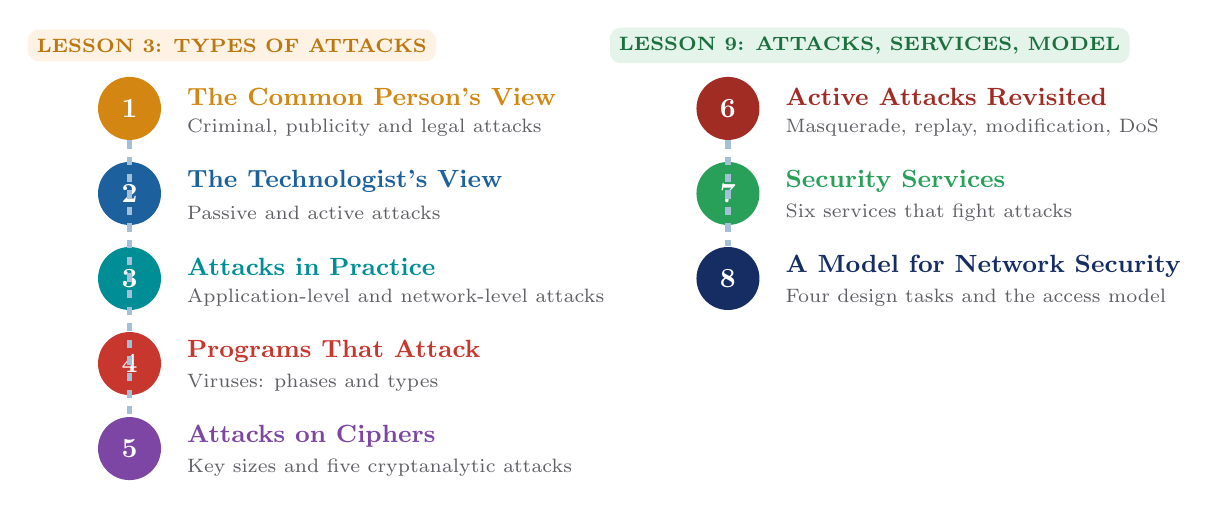
\begin{tikzpicture}
    \foreach \t/\c/\n [count=\i] in {
      The Common Person's View/amber!90!black/Criminal\comma{} publicity and legal attacks,
      The Technologist's View/ocean/Passive and active attacks,
      Attacks in Practice/aqua/Application-level and network-level attacks,
      Programs That Attack/brick/Viruses: phases and types,
      Attacks on Ciphers/grape/Key sizes and five cryptanalytic attacks,
      Active Attacks Revisited/brick!80!black/Masquerade\comma{} replay\comma{} modification\comma{} DoS,
      Security Services/leaf/Six services that fight attacks,
      A Model for Network Security/navy/Four design tasks and the access model}
    {
      \pgfmathsetmacro{\x}{ifthenelse(\i<6,0,7.6)}
      \pgfmathsetmacro{\y}{ifthenelse(\i<6,-(\i-1)*1.08,-(\i-6)*1.08)}
      \node[circle,fill=\c,text=white,font=\bfseries,minimum size=8mm] (n\i) at (\x,\y) {\i};
      \node[anchor=west,font=\small\bfseries,text=\c] at ([xshift=2mm,yshift=1.5mm]n\i.east) {\t};
      \node[anchor=west,font=\scriptsize,text=ink!75] at ([xshift=2mm,yshift=-2.4mm]n\i.east) {\n};
    }
    \draw[ocean!40,line width=2pt,dashed] (n1) -- (n5);
    \draw[ocean!40,line width=2pt,dashed] (n6) -- (n8);
    \node[fill=amber!12,rounded corners,font=\scriptsize\bfseries,text=amber!80!black] at (1.3,0.8) {LESSON 3: TYPES OF ATTACKS};
    \node[fill=leaf!12,rounded corners,font=\scriptsize\bfseries,text=leaf!70!black] at (9.4,0.8) {LESSON 9: ATTACKS, SERVICES, MODEL};
  \end{tikzpicture}
\end{frame}

% ============================================================
\setcounter{section}{2}
\section{Types of Attacks}
% ============================================================

\begin{frame}{Two Ways to Look at Attacks}
  \centering
  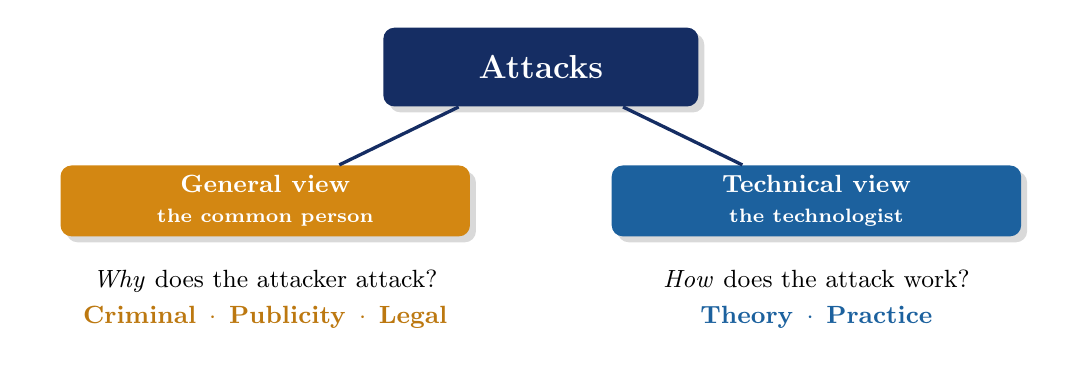
\begin{tikzpicture}[level distance=17mm,level 1/.style={sibling distance=70mm},
      edge from parent/.style={draw=navy,very thick}]
    \node[solid box=navy,minimum width=40mm,minimum height=10mm,font=\large\bfseries] {Attacks}
      child {node[solid box=amber!90!black,minimum width=52mm,minimum height=9mm] (g) {General view\\\scriptsize the common person}}
      child {node[solid box=ocean,minimum width=52mm,minimum height=9mm] (t) {Technical view\\\scriptsize the technologist}};
    \node[below=3mm of g,text width=58mm,align=center,font=\small] {\emph{Why} does the attacker attack?\\[2pt]
      \textcolor{amber!80!black}{\textbf{Criminal} \,$\cdot$\, \textbf{Publicity} \,$\cdot$\, \textbf{Legal}}};
    \node[below=3mm of t,text width=58mm,align=center,font=\small] {\emph{How} does the attack work?\\[2pt]
      \textcolor{ocean}{\textbf{Theory} \,$\cdot$\, \textbf{Practice}}};
  \end{tikzpicture}
  \vspace{4mm}
  \begin{block}{Why two views?}
    \small A bank manager worries about \emph{fraud}; a network engineer worries about \emph{packet modification}.
    Both describe the same threat, from different angles.
  \end{block}
\end{frame}

% ------------------------------------------------------------
\begin{frame}{The General View: Three Categories}
  \centering
  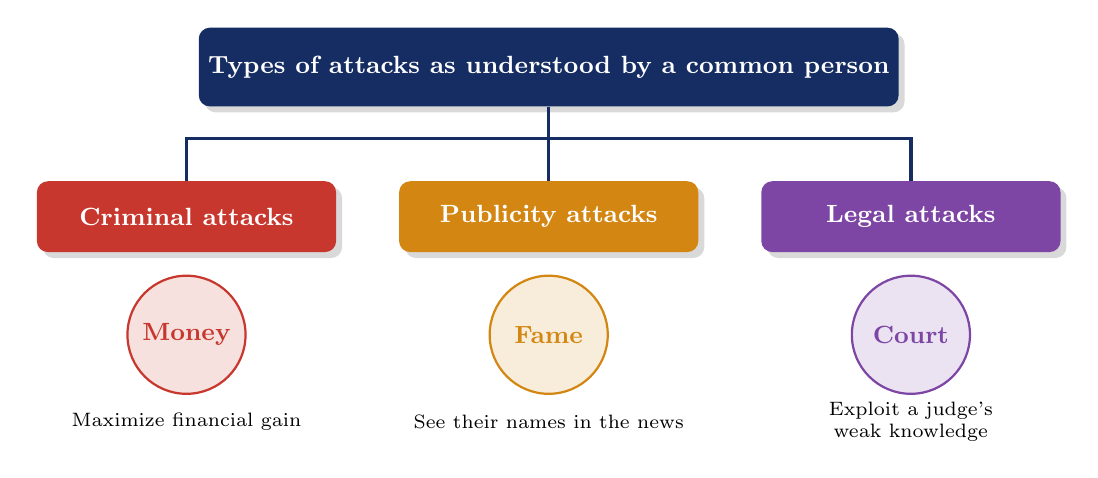
\begin{tikzpicture}
    \node[solid box=navy,minimum width=58mm,minimum height=10mm] (top) at (0,0) {Types of attacks as understood by a common person};
    \foreach \x/\c/\t/\m/\d [count=\k] in {
      -4.6/brick/Criminal attacks/Money/Maximize financial gain,
      0/amber!90!black/Publicity attacks/Fame/See their names in the news,
      4.6/grape/Legal attacks/Court/Exploit a judge's weak knowledge}
    {
      \node[solid box=\c,minimum width=38mm,minimum height=9mm] (b\k) at (\x,-1.9) {\t};
      \draw[navy,very thick] (top.south) -- ++(0,-0.4) -| (b\k.north);
      \node[circle,fill=\c!15,draw=\c,thick,minimum size=15mm,font=\small\bfseries,text=\c] at (\x,-3.4) {\m};
      \node[font=\scriptsize,text width=38mm,align=center] at (\x,-4.5) {\d};
    }
  \end{tikzpicture}
\end{frame}

% ------------------------------------------------------------
\begin{frame}{Criminal Attacks}
  \begin{columns}[c]
    \begin{column}{0.42\textwidth}
      \centering
      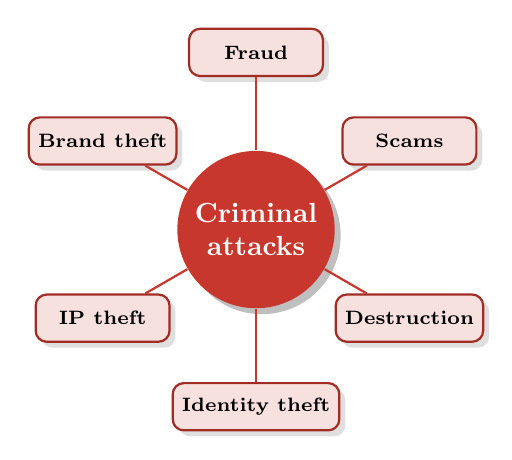
\begin{tikzpicture}
        \node[circle,fill=brick,text=white,font=\bfseries,minimum size=17mm,align=center,drop shadow] (c) at (0,0) {Criminal\\attacks};
        \foreach \a/\t in {90/Fraud,30/Scams,-30/Destruction,-90/Identity theft,-150/IP theft,150/Brand theft}{
          \node[box=brick,minimum width=17mm,minimum height=6mm,font=\scriptsize\bfseries] (s\a) at (\a:2.25) {\t};
          \draw[brick,thick] (c) -- (s\a);
        }
      \end{tikzpicture}
    \end{column}
    \begin{column}{0.56\textwidth}
      \scriptsize
      \renewcommand{\arraystretch}{1.2}
      \begin{tabular}{>{\bfseries\color{brick}}p{1.8cm} >{\raggedright\arraybackslash}p{5.3cm}}
        Fraud & Manipulating e-currency, credit cards, cheques, ATMs \\
        Scams & Fake sales, auctions, ``get rich'' schemes (Nigeria e-mail scam) \\
        Destruction & Grudge attacks by unhappy employees or terrorists (Yahoo!, CNN, eBay in 2000) \\
        Identity theft & \emph{Becoming} a legitimate user: stolen bank passwords, cards in someone's name \\
        IP theft & Stealing trade secrets, databases, music, videos, software \\
        Brand theft & Fake look-alike web sites that collect users' secrets \\
      \end{tabular}
      \vspace{1mm}

      \begin{alertblock}{Goal}
        \small The only aim is to \textbf{maximize financial gain}.
      \end{alertblock}
    \end{column}
  \end{columns}
\end{frame}

% ------------------------------------------------------------
\begin{frame}{Publicity Attacks}
  \begin{columns}[c]
    \begin{column}{0.5\textwidth}
      \centering
      
\begin{tikzpicture}
        % browser window
        \draw[navy,very thick,rounded corners=3pt,fill=white] (0,0) rectangle (5.2,3.4);
        \fill[navy] (0,3.0) [rounded corners=3pt] -- (0,3.4) -- (5.2,3.4) -- (5.2,3.0) [sharp corners] -- cycle;
        \foreach \x/\c in {0.2/brick,0.42/amber,0.64/leaf} \fill[\c] (\x,3.2) circle (0.07);
        \node[fill=white,font=\tiny,minimum width=30mm,inner sep=1pt] at (3.0,3.2) {www.department.gov};
        \node[font=\Large\bfseries,text=brick,rotate=8] at (2.6,1.9) {HACKED!};
        \node[font=\scriptsize\bfseries,text=brick,rotate=8] at (2.6,1.3) {by ``the famous group''};
        \foreach \y in {0.45,0.7} \draw[ink!20,line width=3pt] (0.4,\y) -- (4.8,\y);
        \pic at (6.1,1.7) {person=brick};
        \node[tag,text=brick] at (6.1,1.1) {``Look at me!''};
      \end{tikzpicture}
    \end{column}
    \begin{column}{0.48\textwidth}
      \begin{itemize}\setlength{\itemsep}{5pt}\small
        \item Attackers want to see their \textbf{names on TV and in newspapers}
        \item Usually \textbf{not hardcore criminals}: often students or employees seeking publicity with a novel attack
        \item Common form: \textbf{defacing web pages}
      \end{itemize}
      \vspace{2mm}
      \begin{exampleblock}{Famous cases}
        \small \textbullet~US Department of Justice web site (1996)\\
        \textbullet~\emph{The New York Times} home page (two years later)
      \end{exampleblock}
    \end{column}
  \end{columns}
\end{frame}

% ------------------------------------------------------------
\begin{frame}{Legal Attacks}
  \centering
  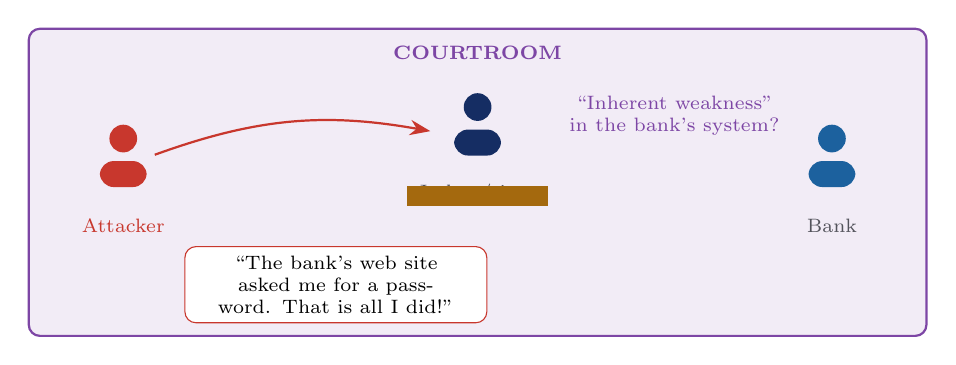
\begin{tikzpicture}
    % courtroom
    \fill[grape!10,draw=grape,thick,rounded corners] (-1.2,-2.0) rectangle (10.2,1.9);
    \node[font=\scriptsize\bfseries,text=grape] at (4.5,1.6) {COURTROOM};
    \pic[scale=1.1] at (0,0) {person=brick}; \node[tag,text=brick] at (0,-0.6) {Attacker};
    \pic[scale=1.1] at (4.5,0.4) {person=navy}; \node[tag] at (4.5,-0.2) {Judge / jury};
    \fill[amber!70!black] (3.6,-0.35) rectangle (5.4,-0.1);
    \pic[scale=1.1] at (9,0) {person=ocean}; \node[tag] at (9,-0.6) {Bank};
    \node[draw=brick,fill=white,rounded corners,font=\scriptsize,text width=36mm,align=center] (q) at (2.7,-1.35)
      {``The bank's web site asked me for a password. That is all I did!''};
    \draw[->,brick,thick] (0.4,0.3) to[bend left=15] (3.9,0.6);
    \node[font=\scriptsize,text=grape,align=center] at (7.0,0.8) {``Inherent weakness''\\in the bank's system?};
  \end{tikzpicture}
  \vspace{3mm}
  \begin{columns}[T]
    \begin{column}{0.5\textwidth}
      \begin{itemize}\small
        \item A \textbf{novel and unique} form of attack
        \item The attacker makes the judge doubt the \textbf{security of a computer system}
      \end{itemize}
    \end{column}
    \begin{column}{0.46\textwidth}
      \begin{alertblock}{The trick}
        \small Exploit the weak technology knowledge of the \textbf{judge and jury}, who are likely to sympathize with the attacker.
      \end{alertblock}
    \end{column}
  \end{columns}
\end{frame}

% ------------------------------------------------------------
\begin{frame}{The Technical View}
  \centering
  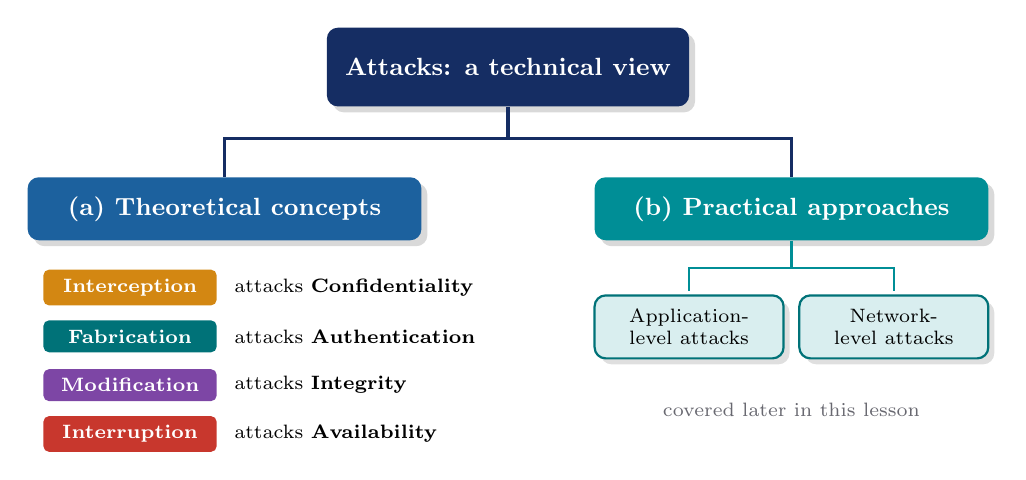
\begin{tikzpicture}
    \node[solid box=navy,minimum width=46mm,minimum height=10mm] (t) at (0,0) {Attacks: a technical view};
    \node[solid box=ocean,minimum width=50mm] (a) at (-3.6,-1.8) {(a) Theoretical concepts};
    \node[solid box=aqua,minimum width=50mm] (b) at (3.6,-1.8) {(b) Practical approaches};
    \draw[navy,very thick] (t.south) -- ++(0,-0.4) -| (a.north);
    \draw[navy,very thick] (t.south) -- ++(0,-0.4) -| (b.north);
    \foreach \t/\c/\g [count=\i from 0] in {Interception/amber!90!black/Confidentiality,Fabrication/aqua!80!black/Authentication,Modification/grape/Integrity,Interruption/brick/Availability}{
      \node[fill=\c,text=white,rounded corners=2pt,font=\scriptsize\bfseries,minimum width=22mm] at (-4.8,-2.8-\i*0.62) {\t};
      \node[font=\scriptsize,anchor=west] at (-3.6,-2.8-\i*0.62) {attacks \textbf{\g}};
    }
    \node[box=aqua,minimum width=24mm,font=\scriptsize] at (2.3,-3.3) {Application-\\level attacks};
    \node[box=aqua,minimum width=24mm,font=\scriptsize] at (4.9,-3.3) {Network-\\level attacks};
    \draw[aqua,thick] (b.south) -- ++(0,-0.35) -| (2.3,-2.85);
    \draw[aqua,thick] (b.south) -- ++(0,-0.35) -| (4.9,-2.85);
    \node[font=\scriptsize,text=ink!70,text width=50mm,align=center] at (3.6,-4.35) {covered later in this lesson};
  \end{tikzpicture}
\end{frame}

% ------------------------------------------------------------
\begin{frame}{Passive and Active Attacks}
  \begin{columns}[c]
    \begin{column}{0.5\textwidth}
      \centering
      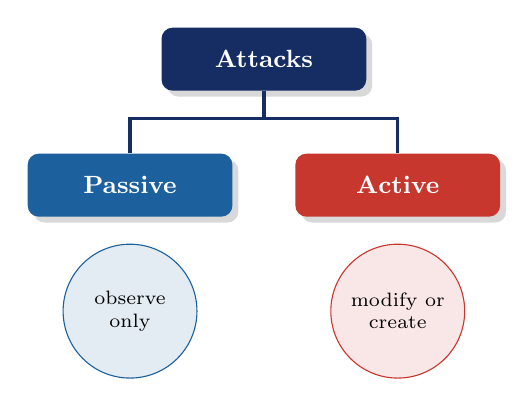
\begin{tikzpicture}
        \node[solid box=navy,minimum width=26mm] (a) at (0,0) {Attacks};
        \node[solid box=ocean,minimum width=26mm] (p) at (-1.7,-1.6) {Passive};
        \node[solid box=brick,minimum width=26mm] (c) at (1.7,-1.6) {Active};
        \draw[navy,very thick] (a.south) -- ++(0,-0.35) -| (p.north);
        \draw[navy,very thick] (a.south) -- ++(0,-0.35) -| (c.north);
        \node[circle,fill=ocean!12,draw=ocean,minimum size=17mm,font=\scriptsize,align=center] at (-1.7,-3.2) {observe\\only};
        \node[circle,fill=brick!12,draw=brick,minimum size=17mm,font=\scriptsize,align=center] at (1.7,-3.2) {modify or\\create};
      \end{tikzpicture}
    \end{column}
    \begin{column}{0.48\textwidth}
      \begin{block}{Passive attacks}
        \small The intruder \textbf{observes} the message or transmission but does \textbf{not modify} it. The aim is to \textbf{obtain information}.
      \end{block}
      \vspace{1mm}
      \begin{alertblock}{Active attacks}
        \small The \textbf{contents of the original message are modified} in some way, or a false message is created.
      \end{alertblock}
      \vspace{1mm}
      {\small Interception is \textbf{passive}; interruption, modification and fabrication are \textbf{active}.}
    \end{column}
  \end{columns}
\end{frame}

% ------------------------------------------------------------
\begin{frame}{Passive Attack 1: Release of Message Contents}
  \begin{columns}[c]
    \begin{column}{0.52\textwidth}
      \centering
      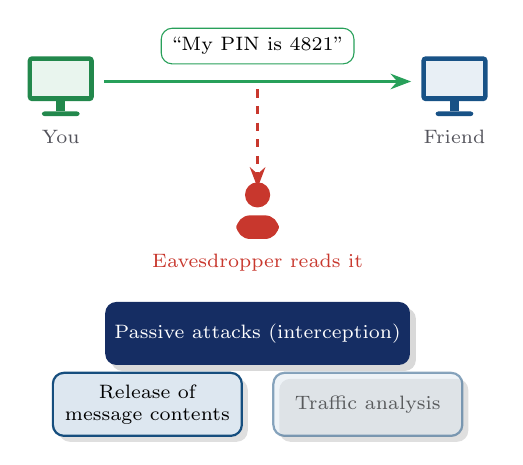
\begin{tikzpicture}
        \pic at (0,0) {pc=leaf}; \node[tag] at (0,-0.5) {You};
        \pic at (5,0) {pc=ocean}; \node[tag] at (5,-0.5) {Friend};
        \draw[flow=leaf] (0.55,0.2) -- (4.45,0.2);
        \node[fill=white,draw=leaf,rounded corners,font=\scriptsize] at (2.5,0.65) {``My PIN is 4821''};
        \pic at (2.5,-1.7) {person=brick}; \node[tag,text=brick] at (2.5,-2.1) {Eavesdropper reads it};
        \draw[brick,dashed,very thick,->] (2.5,0.1) -- (2.5,-1.15);
        \node[solid box=navy,minimum width=26mm,font=\scriptsize] at (2.5,-3.0) {Passive attacks (interception)};
        \node[box=ocean,minimum width=24mm,font=\scriptsize] at (1.1,-3.9) {Release of\\message contents};
        \node[box=ocean,minimum width=24mm,font=\scriptsize,opacity=0.5,text opacity=0.6] at (3.9,-3.9) {Traffic analysis};
      \end{tikzpicture}
    \end{column}
    \begin{column}{0.46\textwidth}
      \begin{itemize}\setlength{\itemsep}{5pt}\small
        \item We send a \textbf{confidential e-mail}: only our friend should read it
        \item If someone else reads it, its contents are \textbf{released against our wishes}
        \item Also: phone calls, transferred files with sensitive data
      \end{itemize}
      \vspace{2mm}
      \begin{exampleblock}{Defence}
        \small \textbf{Encode} the message in a code language (encryption) that only the two parties understand.
      \end{exampleblock}
    \end{column}
  \end{columns}
\end{frame}

% ------------------------------------------------------------
\begin{frame}{Passive Attack 2: Traffic Analysis}
  \begin{columns}[c]
    \begin{column}{0.52\textwidth}
      \centering
      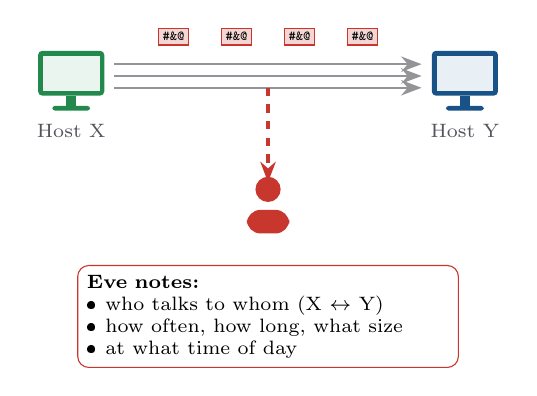
\begin{tikzpicture}
        \pic at (0,0) {pc=leaf}; \node[tag] at (0,-0.5) {Host X};
        \pic at (5,0) {pc=ocean}; \node[tag] at (5,-0.5) {Host Y};
        \foreach \y in {0.05,0.2,0.35} \draw[->,thick,ink!50] (0.55,\y) -- (4.45,\y);
        \foreach \x in {1.3,2.1,2.9,3.7} \node[fill=brick!20,draw=brick,font=\tiny\ttfamily,inner sep=1.5pt] at (\x,0.7) {\#\&@};
        \pic at (2.5,-1.7) {person=brick};
        \draw[brick,dashed,very thick,->] (2.5,0.05) -- (2.5,-1.15);
        \node[draw=brick,fill=white,rounded corners,font=\scriptsize,text width=46mm,align=left,anchor=north] at (2.5,-2.2)
          {\textbf{Eve notes:}\\
           \textbullet~who talks to whom (X $\leftrightarrow$ Y)\\
           \textbullet~how often, how long, what size\\
           \textbullet~at what time of day};
      \end{tikzpicture}
    \end{column}
    \begin{column}{0.46\textwidth}
      \begin{itemize}\setlength{\itemsep}{5pt}\small
        \item Intercepting and examining messages to \textbf{deduce information from patterns}
        \item Works \textbf{even when messages are encrypted} and cannot be read
        \item The more messages observed, the more can be inferred
        \item Reveals the \textbf{location and identity} of communicating hosts
      \end{itemize}
      \vspace{1mm}
      \begin{alertblock}{Example}
        \small A sudden burst of traffic between two companies may reveal a secret merger.
      \end{alertblock}
    \end{column}
  \end{columns}
\end{frame}

% ------------------------------------------------------------
\begin{frame}{Classification of Active Attacks}
  \centering
  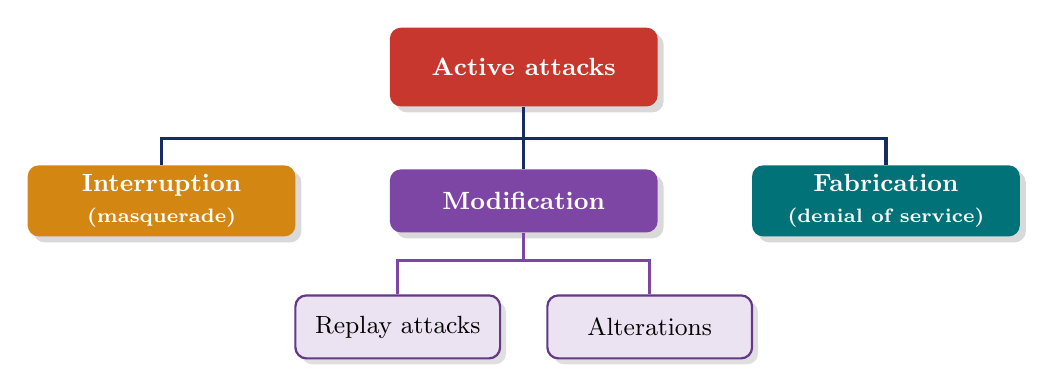
\begin{tikzpicture}
    \node[solid box=brick,minimum width=34mm,minimum height=10mm] (a) at (0,0) {Active attacks};
    \node[solid box=amber!90!black,minimum width=34mm] (i) at (-4.6,-1.7) {Interruption\\\scriptsize(masquerade)};
    \node[solid box=grape,minimum width=34mm] (m) at (0,-1.7) {Modification};
    \node[solid box=aqua!80!black,minimum width=34mm] (f) at (4.6,-1.7) {Fabrication\\\scriptsize(denial of service)};
    \foreach \n in {i,m,f} \draw[navy,very thick] (a.south) -- ++(0,-0.4) -| (\n.north);
    \node[box=grape,minimum width=26mm] (r) at (-1.6,-3.3) {Replay attacks};
    \node[box=grape,minimum width=26mm] (al) at (1.6,-3.3) {Alterations};
    \draw[grape,very thick] (m.south) -- ++(0,-0.35) -| (r.north);
    \draw[grape,very thick] (m.south) -- ++(0,-0.35) -| (al.north);
  \end{tikzpicture}
  \vspace{4mm}
  \begin{columns}[T]
    \begin{column}{0.5\textwidth}
      \begin{itemize}\small
        \item Posing as another entity: \textbf{masquerade}
        \item Modification: \textbf{replay} and \textbf{alteration} of messages
      \end{itemize}
    \end{column}
    \begin{column}{0.46\textwidth}
      \begin{itemize}\small
        \item Fabrication: \textbf{denial of service (DoS)}
        \item Cannot be \textbf{prevented} easily, but can be \textbf{detected} and recovered from
      \end{itemize}
    \end{column}
  \end{columns}
\end{frame}

% ------------------------------------------------------------
\begin{frame}{Active Attack: Masquerade}
  \begin{columns}[c]
    \begin{column}{0.52\textwidth}
      \centering
      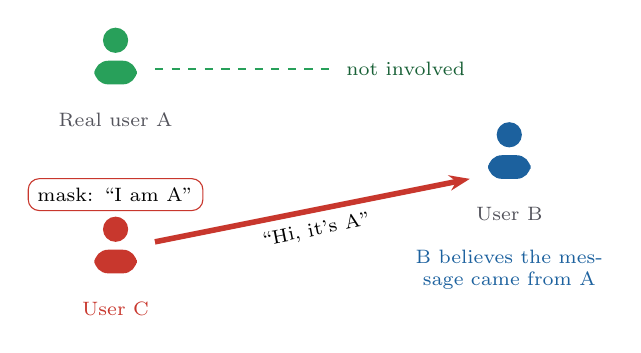
\begin{tikzpicture}
        \pic at (0,1.4) {person=leaf}; \node[tag] at (0,0.85) {Real user A};
        \pic at (0,-1.0) {person=brick}; \node[tag,text=brick] at (0,-1.55) {User C};
        \node[fill=white,draw=brick,rounded corners,font=\scriptsize] at (0,-0.1) {mask: ``I am A''};
        \pic at (5,0.2) {person=ocean}; \node[tag] at (5,-0.35) {User B};
        \draw[flow=brick,line width=2pt] (0.5,-0.7) -- node[below,font=\scriptsize,sloped]{``Hi, it's A''} (4.5,0.1);
        \node[font=\scriptsize,text=ocean,text width=24mm,align=center] at (5,-1.05) {B believes the message came from A};
        \draw[leaf,thick,dashed] (0.5,1.5) -- (2.8,1.5) node[right,font=\scriptsize,text=leaf!60!black]{not involved};
      \end{tikzpicture}
    \end{column}
    \begin{column}{0.46\textwidth}
      \begin{alertblock}{Definition}
        \small An \textbf{unauthorized entity pretends to be another entity}.
      \end{alertblock}
      \vspace{1mm}
      \begin{itemize}\small\setlength{\itemsep}{3pt}
        \item User C sends a message to B posing as user A
        \item Often combined with other active attacks
        \item E.g. capture A's \textbf{user ID and password}, then replay them later to gain illegal access
      \end{itemize}
    \end{column}
  \end{columns}
\end{frame}

% ------------------------------------------------------------
\begin{frame}{Active Attack: Replay}
  \centering
  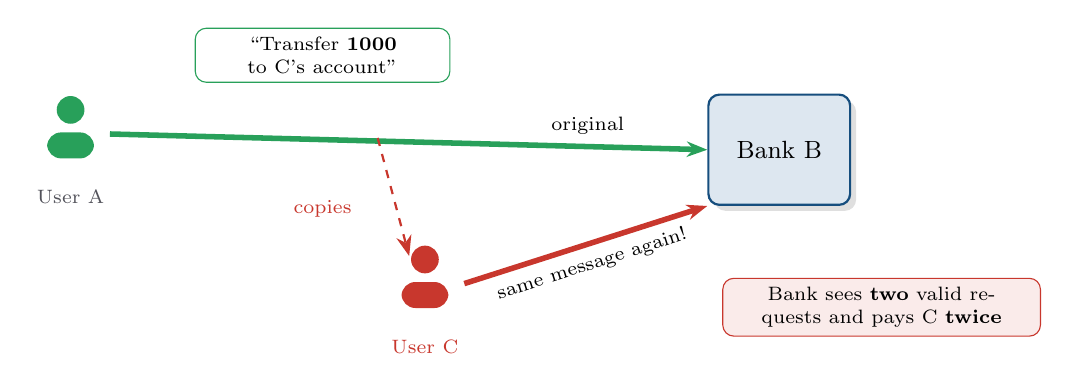
\begin{tikzpicture}
    \pic[scale=1.1] at (0,0) {person=leaf}; \node[tag] at (0,-0.6) {User A};
    \node[box=ocean,minimum width=18mm,minimum height=14mm] (bank) at (9,0) {Bank B};
    \node[fill=white,draw=leaf,rounded corners,font=\scriptsize,text width=30mm,align=center] (msg) at (3.2,1.2) {``Transfer \textbf{1000} to C's account''};
    \draw[flow=leaf,line width=2pt] (0.5,0.2) -- node[above,pos=0.8,font=\scriptsize]{original} (bank.west);
    \pic[scale=1.1] at (4.5,-1.9) {person=brick}; \node[tag,text=brick] at (4.5,-2.5) {User C};
    \draw[brick,dashed,thick,->] (3.9,0.15) -- (4.3,-1.35);
    \node[font=\scriptsize,text=brick] at (3.2,-0.75) {copies};
    \draw[flow=brick,line width=2pt] (5,-1.7) -- node[below,font=\scriptsize,sloped]{same message again!} (bank.south west);
    \node[fill=brick!10,draw=brick,rounded corners,font=\scriptsize,text width=38mm,align=center] at (10.3,-2.0) {Bank sees \textbf{two} valid requests and pays C \textbf{twice}};
  \end{tikzpicture}
  \vspace{3mm}
  \begin{block}{Definition}
    \small A user \textbf{captures a sequence of events or data units and re-sends them}. The bank cannot tell the copy from a second, genuine request.
  \end{block}
\end{frame}

% ------------------------------------------------------------
\begin{frame}{Active Attack: Alteration of Messages}
  \centering
  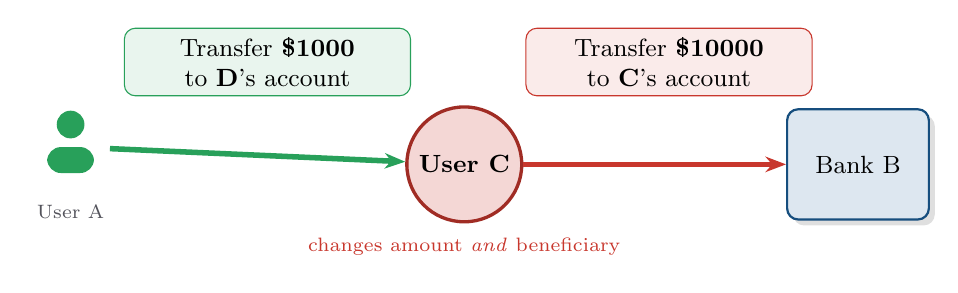
\begin{tikzpicture}
    \pic[scale=1.1] at (0,0) {person=leaf}; \node[tag] at (0,-0.6) {User A};
    \node[box=ocean,minimum width=18mm,minimum height=14mm] (bank) at (10,0) {Bank B};
    \node[station=brick,minimum size=14mm] (c) at (5,0) {User C};
    \draw[flow=leaf,line width=2pt] (0.5,0.2) -- (c);
    \draw[flow=brick,line width=2pt] (c) -- (bank);
    \node[fill=leaf!10,draw=leaf,rounded corners,font=\small,text width=34mm,align=center] at (2.5,1.3) {Transfer \textbf{\$1000} to \textbf{D}'s account};
    \node[fill=brick!10,draw=brick,rounded corners,font=\small,text width=34mm,align=center] at (7.6,1.3) {Transfer \textbf{\$10000} to \textbf{C}'s account};
    \node[font=\scriptsize,text=brick] at (5,-1.05) {changes amount \emph{and} beneficiary};
  \end{tikzpicture}
  \vspace{4mm}
  \begin{columns}[T]
    \begin{column}{0.5\textwidth}
      \begin{alertblock}{Definition}
        \small Some change is made to the \textbf{original message} while it is in transit.
      \end{alertblock}
    \end{column}
    \begin{column}{0.46\textwidth}
      \begin{block}{Note}
        \small Here both the beneficiary and the amount changed; changing \textbf{either one alone} would also be an alteration.
      \end{block}
    \end{column}
  \end{columns}
\end{frame}

% ------------------------------------------------------------
\begin{frame}{Active Attack: Denial of Service (DoS)}
  \begin{columns}[c]
    \begin{column}{0.52\textwidth}
      \centering
      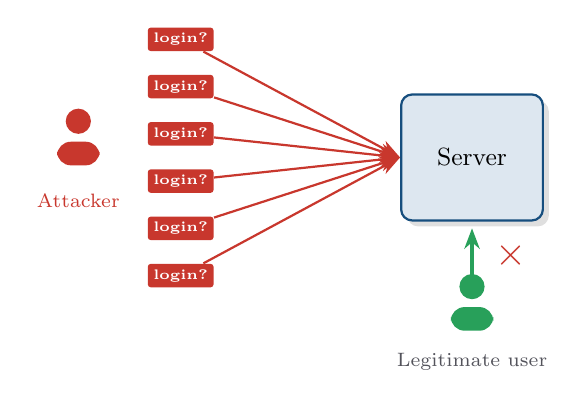
\begin{tikzpicture}
        \node[box=ocean,minimum width=18mm,minimum height=16mm] (srv) at (4.4,0) {Server};
        \foreach \y [count=\i] in {1.5,0.9,0.3,-0.3,-0.9,-1.5}{
          \node[fill=brick,text=white,font=\tiny\bfseries,rounded corners=1pt,inner sep=2pt] (r\i) at (0.7,\y) {login?};
          \draw[->,brick,thick] (r\i) -- (srv.west);
        }
        \pic at (-0.6,0) {person=brick}; \node[tag,text=brick] at (-0.6,-0.55) {Attacker};
        \pic at (4.4,-2.1) {person=leaf}; \node[tag] at (4.4,-2.6) {Legitimate user};
        \draw[leaf,very thick,->] (4.4,-1.55) -- (4.4,-0.9);
        \node[brick,font=\Large\bfseries] at (4.9,-1.25) {$\times$};
      \end{tikzpicture}
    \end{column}
    \begin{column}{0.46\textwidth}
      \begin{alertblock}{Definition}
        \small An attempt to \textbf{prevent legitimate users} from accessing services they are eligible for.
      \end{alertblock}
      \vspace{1mm}
      \textbf{Example}
      \begin{itemize}\small
        \item Send \textbf{too many login requests} with random user IDs in quick succession
        \item The network is \textbf{flooded}
        \item Legitimate users are denied the facilities
      \end{itemize}
      {\small\textbf{Threatens:} \textcolor{grape}{\textbf{availability}}}
    \end{column}
  \end{columns}
\end{frame}

% ------------------------------------------------------------
\begin{frame}{The Practical Side of Attacks}
  \centering
  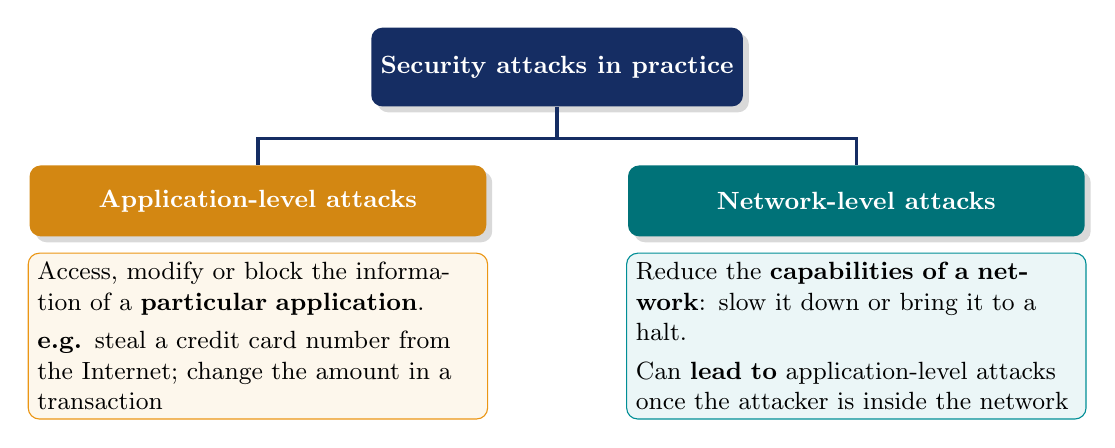
\begin{tikzpicture}
    \node[solid box=navy,minimum width=46mm,minimum height=10mm] (t) at (0,0) {Security attacks in practice};
    \node[solid box=amber!90!black,minimum width=58mm,minimum height=9mm] (a) at (-3.8,-1.7) {Application-level attacks};
    \node[solid box=aqua!80!black,minimum width=58mm,minimum height=9mm] (n) at (3.8,-1.7) {Network-level attacks};
    \draw[navy,very thick] (t.south) -- ++(0,-0.4) -| (a.north);
    \draw[navy,very thick] (t.south) -- ++(0,-0.4) -| (n.north);
    \node[draw=amber,fill=amber!8,rounded corners,text width=56mm,font=\small,anchor=north] at ([yshift=-2mm]a.south)
      {Access, modify or block the information of a \textbf{particular application}.\\[3pt]
       \textbf{e.g.} steal a credit card number from the Internet; change the amount in a transaction};
    \node[draw=aqua,fill=aqua!8,rounded corners,text width=56mm,font=\small,anchor=north] at ([yshift=-2mm]n.south)
      {Reduce the \textbf{capabilities of a network}: slow it down or bring it to a halt.\\[3pt]
       Can \textbf{lead to} application-level attacks once the attacker is inside the network};
  \end{tikzpicture}
  \vspace{3mm}
  \begin{block}{Key sentence}
    \small Security attacks can happen at the \textbf{application level} or at the \textbf{network level}, using many mechanisms.
  \end{block}
\end{frame}

% ------------------------------------------------------------
\begin{frame}{Programs That Attack: The Virus}
  \centering
  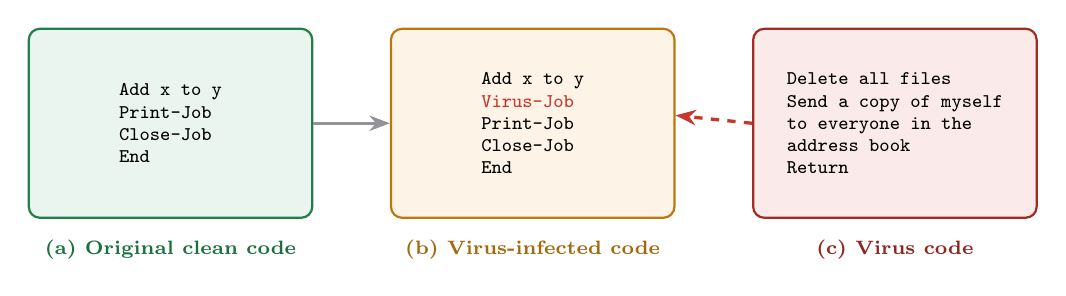
\begin{tikzpicture}
    \foreach \x/\t/\c/\l [count=\k] in {0/{Add x to y\\Print-Job\\Close-Job\\End}/leaf/(a) Original clean code,
                             4.6/{Add x to y\\\textcolor{brick}{\textbf{Virus-Job}}\\Print-Job\\Close-Job\\End}/amber/(b) Virus-infected code,
                             9.2/{Delete all files\\Send a copy of myself\\to everyone in the\\address book\\Return}/brick/(c) Virus code}{
      \node[draw=\c!80!black,fill=\c!10,thick,rounded corners,minimum width=36mm,minimum height=24mm,font=\scriptsize\ttfamily,align=left] (b\k) at (\x,0) {\t};
      \node[font=\scriptsize\bfseries,text=\c!70!black] at (\x,-1.6) {\l};
    }
    \draw[flow=ink!50] (b1) -- (b2);
    \draw[flow=brick,dashed] (b3.west) -- ([yshift=1mm]b2.east);
  \end{tikzpicture}
  \vspace{3mm}
  \begin{columns}[T]
    \begin{column}{0.5\textwidth}
      \begin{block}{Definition}
        \small A computer program that \textbf{attaches itself to another legitimate program} and causes damage to the computer system or network.
      \end{block}
    \end{column}
    \begin{column}{0.46\textwidth}
      \begin{itemize}\small
        \item Runs whenever the host program runs
        \item Can infect other programs on the same computer or network
        \item Can be triggered by events (e.g. 12 PM every day)
      \end{itemize}
    \end{column}
  \end{columns}
\end{frame}

% ------------------------------------------------------------
\begin{frame}{The Four Phases of a Virus}
  \centering
  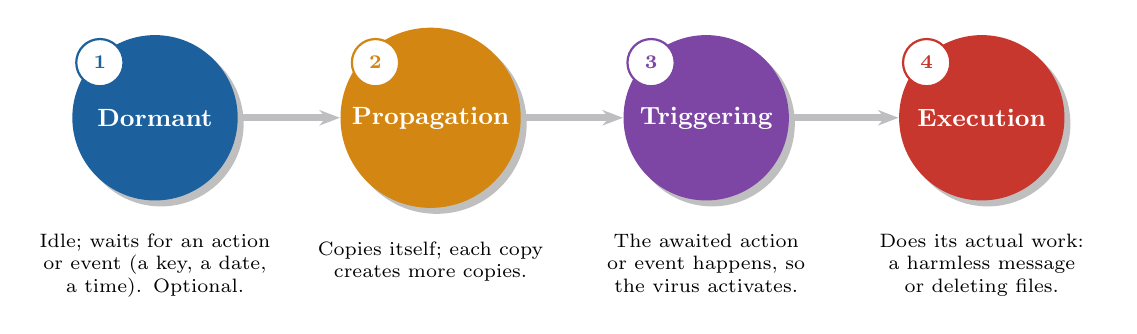
\begin{tikzpicture}
    \foreach \t/\c/\d [count=\i from 0] in {
      Dormant/ocean/Idle; waits for an action or event (a key\comma{} a date\comma{} a time). Optional.,
      Propagation/amber!90!black/Copies itself; each copy creates more copies.,
      Triggering/grape/The awaited action or event happens\comma{} so the virus activates.,
      Execution/brick/Does its actual work: a harmless message or deleting files.}
    {
      \node[circle,fill=\c,text=white,font=\small\bfseries,minimum size=21mm,drop shadow] (p\i) at (\i*3.5,0) {\t};
      \node[font=\scriptsize,text width=30mm,align=center,below=3mm of p\i] {\d};
      \node[circle,fill=white,draw=\c,thick,font=\scriptsize\bfseries,text=\c,minimum size=6mm] at ([xshift=-7mm,yshift=7mm]p\i) {\the\numexpr\i+1\relax};
    }
    \foreach \i [evaluate=\i as \j using int(\i+1)] in {0,1,2} \draw[->,line width=2.5pt,ink!30] (p\i) -- (p\j);
  \end{tikzpicture}
  \vspace{3mm}
  \begin{block}{Good news}
    \small Usually the damage can be repaired, provided the organization keeps \textbf{good backup and recovery} procedures.
  \end{block}
\end{frame}

% ------------------------------------------------------------
\begin{frame}{Types of Viruses}
  \centering
  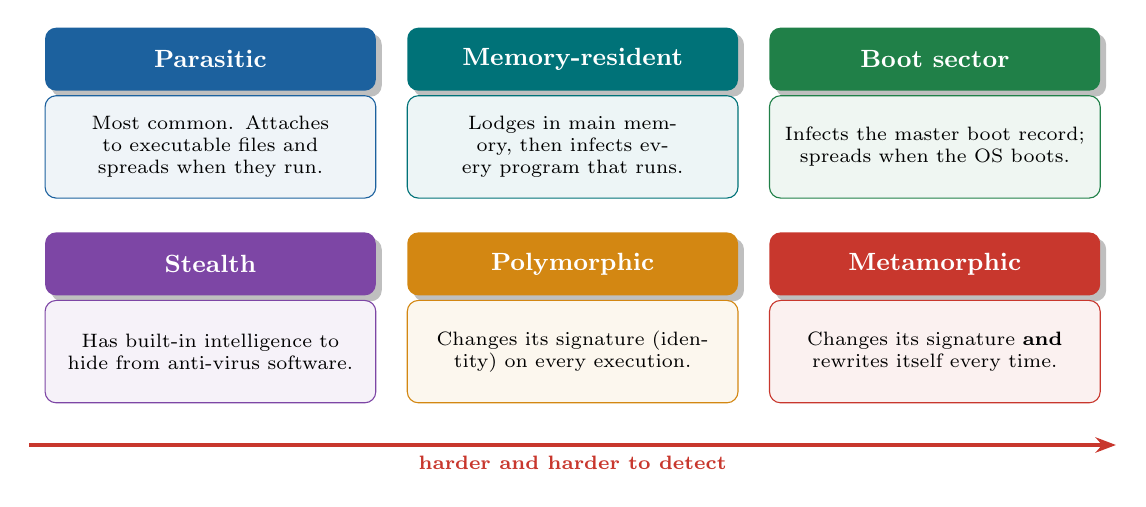
\begin{tikzpicture}
    \foreach \t/\d/\c [count=\i from 0] in {
      Parasitic/Most common. Attaches to executable files and spreads when they run./ocean,
      Memory-resident/Lodges in main memory\comma{} then infects every program that runs./aqua!80!black,
      Boot sector/Infects the master boot record; spreads when the OS boots./leaf!80!black,
      Stealth/Has built-in intelligence to hide from anti-virus software./grape,
      Polymorphic/Changes its signature (identity) on every execution./amber!90!black,
      Metamorphic/Changes its signature \textbf{and} rewrites itself every time./brick}
    {
      \pgfmathsetmacro{\x}{mod(\i,3)*4.6}
      \pgfmathsetmacro{\y}{-floor(\i/3)*2.6}
      \node[fill=\c,text=white,font=\small\bfseries,rounded corners=4pt,minimum width=42mm,minimum height=8mm,drop shadow] (h\i) at (\x,\y) {\t};
      \node[draw=\c,fill=\c!7,rounded corners=4pt,minimum width=42mm,minimum height=13mm,text width=39mm,align=center,font=\scriptsize,anchor=north] at ([yshift=-0.5mm]h\i.south) {\d};
    }
    \draw[->,very thick,brick] (-2.3,-4.9) -- node[below,font=\scriptsize\bfseries,text=brick]{harder and harder to detect} (11.5,-4.9);
  \end{tikzpicture}
\end{frame}

% ------------------------------------------------------------
\begin{frame}{Key Sizes and Ranges}
  \begin{columns}[c]
    \begin{column}{0.55\textwidth}
      \centering
      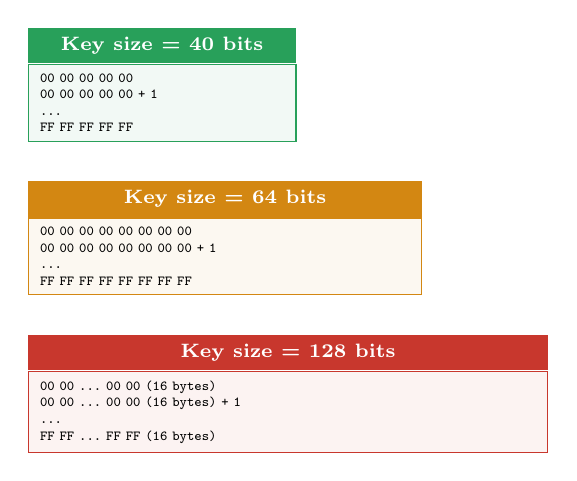
\begin{tikzpicture}
        \foreach \b/\w/\c/\first/\last [count=\i from 0] in {
          40/34/leaf/00 00 00 00 00/FF FF FF FF FF,
          64/50/amber!90!black/00 00 00 00 00 00 00 00/FF FF FF FF FF FF FF FF,
          128/66/brick/00 00 \dots\ 00 00 (16 bytes)/FF FF \dots\ FF FF (16 bytes)}{
          \node[fill=\c,text=white,font=\scriptsize\bfseries,minimum width=\w mm,anchor=west] (h\i) at (0,-\i*1.95) {Key size = \b\ bits};
          \node[draw=\c,fill=\c!6,minimum width=\w mm,anchor=north west,font=\tiny\ttfamily,align=left,text width=\w mm - 3mm] at (h\i.south west) {\first\\ \first{} + 1\\ \dots\\ \last};
        }
      \end{tikzpicture}
    \end{column}
    \begin{column}{0.43\textwidth}
      \begin{itemize}\small\setlength{\itemsep}{4pt}
        \item Keys can be written in \textbf{hexadecimal}
        \item Bigger key $\Rightarrow$ bigger range $\Rightarrow$ more work for the attacker
        \item $2^{128} \approx 3.4\times10^{38}$ possible keys
        \item 56-bit keys are no longer safe; 128-bit is safe \emph{today}
      \end{itemize}
      \vspace{2mm}
      \begin{exampleblock}{Will 512 bits ever break?}
        \small Even if every atom in the universe ($2^{300}$) were a computer checking $2^{300}$ keys/s, searching 1\% of a 512-bit space would take $2^{162}$ millennia. The universe is younger than $2^{34}$ millennia!
      \end{exampleblock}
    \end{column}
  \end{columns}
\end{frame}

% ------------------------------------------------------------
\begin{frame}{Possible Types of Attacks on a Cipher}
  \centering
  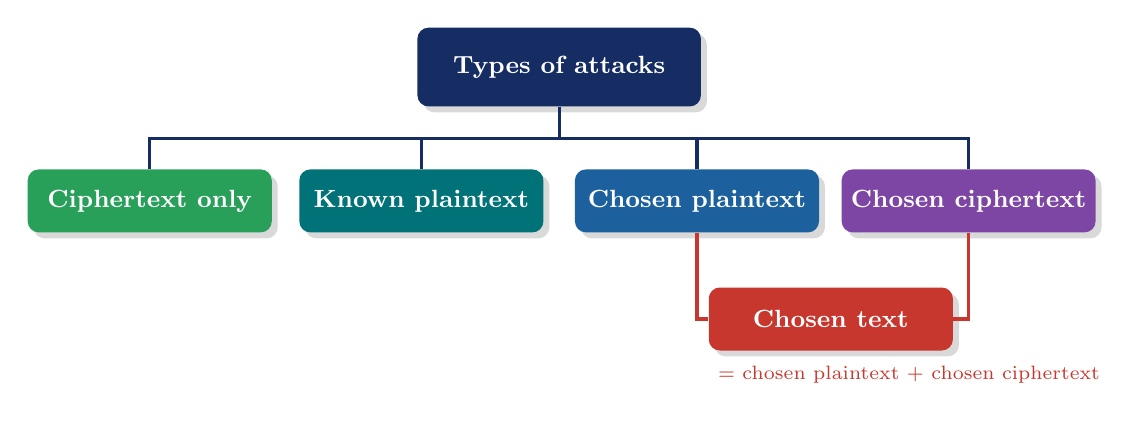
\begin{tikzpicture}
    \node[solid box=navy,minimum width=36mm,minimum height=10mm] (t) at (0,0) {Types of attacks};
    \foreach \t/\c/\x [count=\i] in {Ciphertext only/leaf/-5.2,Known plaintext/aqua!80!black/-1.75,Chosen plaintext/ocean/1.75,Chosen ciphertext/grape/5.2}{
      \node[solid box=\c,minimum width=31mm] (n\i) at (\x,-1.7) {\t};
      \draw[navy,very thick] (t.south) -- ++(0,-0.4) -| (n\i.north);
    }
    \node[solid box=brick,minimum width=31mm] (ct) at (3.45,-3.2) {Chosen text};
    \draw[brick,very thick] (n3.south) |- (ct.west);
    \draw[brick,very thick] (n4.south) |- (ct.east);
    \node[font=\scriptsize,text=brick,anchor=west] at (ct.south west) [yshift=-3mm] {= chosen plaintext + chosen ciphertext};
  \end{tikzpicture}
  \vspace{3mm}
  \begin{block}{The setting}
    \small The sender encrypts a plaintext message into ciphertext. The attacker's goal is to find the \textbf{plaintext} or, better, the \textbf{key}. What the attacker already knows decides which of these \textbf{five} attacks is possible.
  \end{block}
\end{frame}

% ------------------------------------------------------------
\begin{frame}{Ciphertext-Only Attack}
  \begin{columns}[c]
    \begin{column}{0.52\textwidth}
      \centering
      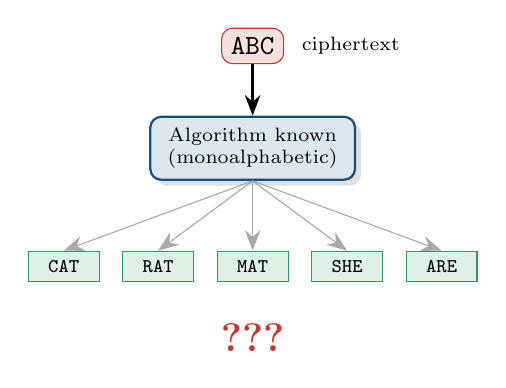
\begin{tikzpicture}
        \node[fill=brick!15,draw=brick,rounded corners,font=\ttfamily\bfseries] (c) at (2.4,1.5) {ABC};
        \node[font=\scriptsize,right=1mm of c] {ciphertext};
        \node[box=ocean,minimum width=26mm,font=\scriptsize] (alg) at (2.4,0.2) {Algorithm known\\(monoalphabetic)};
        \draw[->,very thick] (c) -- (alg);
        \foreach \w/\x [count=\k] in {CAT/0,RAT/1.2,MAT/2.4,SHE/3.6,ARE/4.8}{
          \node[fill=leaf!15,draw=leaf,font=\scriptsize\ttfamily,minimum width=9mm] (w\k) at (\x,-1.3) {\w};
          \draw[->,ink!40] (alg.south) -- (w\k.north);
        }
        \node[font=\Large\bfseries,text=brick] at (2.4,-2.2) {???};
      \end{tikzpicture}
    \end{column}
    \begin{column}{0.46\textwidth}
      \begin{itemize}\small\setlength{\itemsep}{4pt}
        \item The attacker has \textbf{only ciphertext} and no clue about the plaintext
        \item Analyses it using \textbf{letter frequencies} (e, i, a are common in English)
        \item \textbf{More ciphertext} means better chances
      \end{itemize}
      \vspace{2mm}
      \begin{alertblock}{Confusion for the attacker}
        \small A short block like \texttt{ABC} could be CAT, RAT, MAT, SHE, ARE\dots: far too many possibilities.
      \end{alertblock}
    \end{column}
  \end{columns}
\end{frame}

% ------------------------------------------------------------
\begin{frame}{Known-Plaintext Attack}
  \begin{columns}[c]
    \begin{column}{0.52\textwidth}
      \centering
      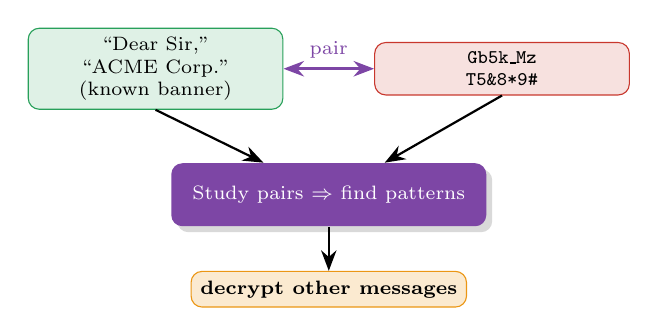
\begin{tikzpicture}
        \node[fill=leaf!15,draw=leaf,rounded corners,font=\scriptsize,text width=30mm,align=center] (p) at (0,1.2) {``Dear Sir,''\\``ACME Corp.''\\(known banner)};
        \node[fill=brick!15,draw=brick,rounded corners,font=\scriptsize\ttfamily,text width=30mm,align=center] (c) at (4.4,1.2) {Gb5k\_Mz\\T5\&8*9\#};
        \draw[<->,very thick,grape] (p) -- node[above,font=\scriptsize]{pair} (c);
        \node[solid box=grape,minimum width=40mm,font=\scriptsize] (k) at (2.2,-0.4) {Study pairs $\Rightarrow$ find patterns};
        \draw[->,thick] (p.south) -- (k); \draw[->,thick] (c.south) -- (k);
        \node[fill=amber!20,draw=amber,rounded corners,font=\scriptsize\bfseries] (r) at (2.2,-1.6) {decrypt other messages};
        \draw[->,thick] (k) -- (r);
      \end{tikzpicture}
    \end{column}
    \begin{column}{0.46\textwidth}
      \begin{itemize}\small\setlength{\itemsep}{4pt}
        \item The attacker knows some \textbf{plaintext--ciphertext pairs}
        \item Uses them to find \textbf{more pairs} and more plaintext
        \item Examples: company banners, file headers, standard greetings
      \end{itemize}
      \vspace{2mm}
      \begin{block}{How does the attacker get plaintext?}
        \small Old plaintext may become \textbf{outdated and public}, or be \textbf{leaked} inadvertently.
      \end{block}
    \end{column}
  \end{columns}
\end{frame}

% ------------------------------------------------------------
\begin{frame}{Chosen-Plaintext Attack: The Telegraph Story}
  \centering
  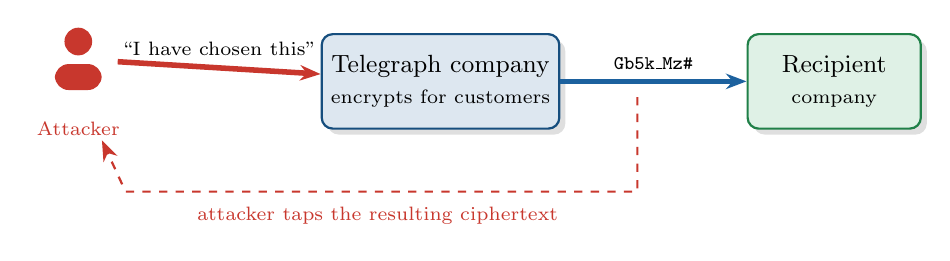
\begin{tikzpicture}
    \pic[scale=1.1] at (0,0) {person=brick}; \node[tag,text=brick] at (0,-0.6) {Attacker};
    \node[box=ocean,minimum width=30mm,minimum height=12mm] (tel) at (4.6,0) {Telegraph company\\\scriptsize encrypts for customers};
    \node[box=leaf,minimum width=22mm,minimum height=12mm] (dst) at (9.6,0) {Recipient\\\scriptsize company};
    \draw[flow=brick,line width=2pt] (0.5,0.25) -- node[above,font=\scriptsize]{``I have chosen this''} (tel);
    \draw[flow=ocean,line width=2pt] (tel) -- node[above,font=\scriptsize]{\texttt{Gb5k\_Mz\#}} (dst);
    \draw[brick,dashed,thick,->] (7.1,-0.2) -- (7.1,-1.4) -- (0.6,-1.4) -- (0.3,-0.75);
    \node[font=\scriptsize,text=brick] at (3.8,-1.7) {attacker taps the resulting ciphertext};
  \end{tikzpicture}
  \vspace{3mm}
  \begin{columns}[T]
    \begin{column}{0.5\textwidth}
      \begin{block}{Definition}
        \small The attacker \textbf{selects a plaintext block} and obtains its ciphertext, deliberately picking patterns that reveal more about the key.
      \end{block}
    \end{column}
    \begin{column}{0.46\textwidth}
      \begin{itemize}\small
        \item A telegraph company encrypts people's messages for them
        \item The attacker simply \textbf{pays} to send a chosen text
        \item Now they own a matching plaintext--ciphertext pair
      \end{itemize}
    \end{column}
  \end{columns}
\end{frame}

% ------------------------------------------------------------
\begin{frame}{Chosen-Ciphertext and Chosen-Text Attacks}
  \begin{columns}[T]
    \begin{column}{0.49\textwidth}
      \centering
      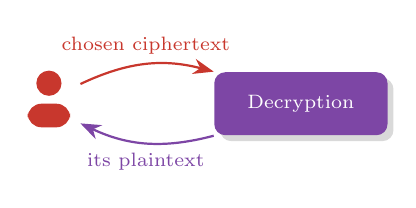
\begin{tikzpicture}
        \pic at (0,0) {person=brick};
        \node[solid box=grape,minimum width=22mm,font=\scriptsize] (o) at (3.2,0.2) {Decryption};
        \draw[->,thick,brick] (0.4,0.45) to[bend left=20] node[above,font=\scriptsize]{chosen ciphertext} (o.north west);
        \draw[->,thick,grape] (o.south west) to[bend left=20] node[below,font=\scriptsize]{its plaintext} (0.4,-0.05);
      \end{tikzpicture}
      \begin{block}{Chosen ciphertext}
        \small The attacker knows the ciphertext to be decrypted, the \textbf{algorithm}, and the corresponding plaintext block. The job: \textbf{discover the key}. Not very common.
      \end{block}
    \end{column}
    \begin{column}{0.49\textwidth}
      \centering
      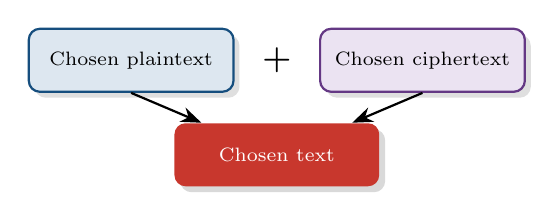
\begin{tikzpicture}
        \node[box=ocean,minimum width=26mm,font=\scriptsize] (a) at (0,0.6) {Chosen plaintext};
        \node[font=\large\bfseries] at (1.85,0.6) {+};
        \node[box=grape,minimum width=26mm,font=\scriptsize] (b) at (3.7,0.6) {Chosen ciphertext};
        \node[solid box=brick,minimum width=26mm,font=\scriptsize] (c) at (1.85,-0.6) {Chosen text};
        \draw[->,thick] (a.south) -- (c); \draw[->,thick] (b.south) -- (c);
      \end{tikzpicture}
      \begin{alertblock}{Chosen text}
        \small Essentially a \textbf{combination} of the chosen-plaintext and chosen-ciphertext attacks.
      \end{alertblock}
    \end{column}
  \end{columns}
\end{frame}

% ------------------------------------------------------------
\begin{frame}{Summary of Attacks on Ciphers}
  \centering
  \scriptsize
  \renewcommand{\arraystretch}{1.3}
  \begin{tabular}{>{\bfseries}p{2.3cm} p{5.4cm} p{4.3cm}}
    \toprule
    \rowcolor{navy}\textcolor{white}{Attack} & \textcolor{white}{\textbf{Things known to the attacker}} & \textcolor{white}{\textbf{Things the attacker wants}}\\
    \midrule
    \rowcolor{leaf!8}\textcolor{leaf!70!black}{Ciphertext only} & Ciphertext of several messages (same key); algorithm & Plaintext of those messages; the key\\
    \rowcolor{aqua!8}\textcolor{aqua!70!black}{Known plaintext} & Ciphertext of several messages; some matching plaintext; algorithm & Algorithm to decrypt; the key\\
    \rowcolor{ocean!8}\textcolor{ocean}{Chosen plaintext} & Ciphertext and plaintext; chooses the plaintext to encrypt & The key; decryption of other ciphertext\\
    \rowcolor{grape!8}\textcolor{grape}{Chosen ciphertext} & Ciphertext of messages to be decrypted; matching plaintext & The key used for encryption\\
    \rowcolor{brick!8}\textcolor{brick}{Chosen text} & Some of the above & Some of the above\\
    \bottomrule
  \end{tabular}
  \vspace{4mm}

  
\begin{tikzpicture}
    \node[fill=sky,rounded corners,text width=12cm,align=center,font=\small,inner sep=6pt]
      {Reading down the table, the attacker \textbf{knows more}, so the attack becomes \textbf{more powerful}.};
  \end{tikzpicture}
\end{frame}

% ============================================================
\setcounter{section}{8}
\section{Cryptography: Attacks, Services and the Security Model}
% ============================================================

\begin{frame}{Quick Recap from Module 1}
  \begin{columns}[c]
    \begin{column}{0.5\textwidth}
      \centering
      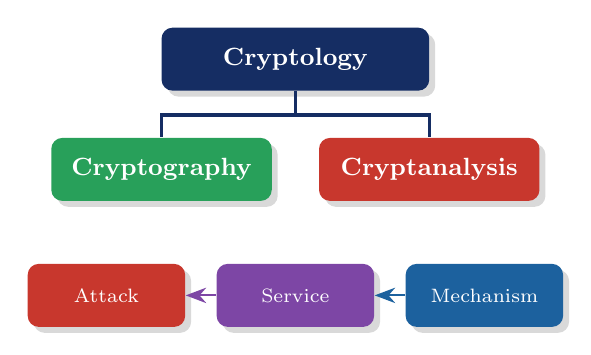
\begin{tikzpicture}
        \node[solid box=navy,minimum width=34mm] (cy) at (0,0) {Cryptology};
        \node[solid box=leaf,minimum width=28mm] (cg) at (-1.7,-1.4) {Cryptography};
        \node[solid box=brick,minimum width=28mm] (ca) at (1.7,-1.4) {Cryptanalysis};
        \draw[navy,very thick] (cy.south) -- ++(0,-0.3) -| (cg.north);
        \draw[navy,very thick] (cy.south) -- ++(0,-0.3) -| (ca.north);
        \node[solid box=brick,minimum width=20mm,font=\scriptsize] (a) at (-2.4,-3.0) {Attack};
        \node[solid box=grape,minimum width=20mm,font=\scriptsize] (s) at (0,-3.0) {Service};
        \node[solid box=ocean,minimum width=20mm,font=\scriptsize] (m) at (2.4,-3.0) {Mechanism};
        \draw[<-,thick,grape] (a) -- (s); \draw[<-,thick,ocean] (s) -- (m);
      \end{tikzpicture}
    \end{column}
    \begin{column}{0.48\textwidth}
      \begin{itemize}\small\setlength{\itemsep}{4pt}
        \item \textbf{Cryptography}: designing systems to code and decode messages
        \item \textbf{Cryptanalysis}: breaking them without the key
        \item \textbf{Attack}: compromises security
        \item \textbf{Mechanism}: detects, prevents or recovers (encryption, digital signature, SSL)
        \item \textbf{Service}: enhances security, using one or more mechanisms
      \end{itemize}
      \vspace{1mm}
      {\small\textcolor{ink!70}{Lesson 9 now looks deeper at attacks, services and a \textbf{model} that ties them together.}}
    \end{column}
  \end{columns}
\end{frame}

% ------------------------------------------------------------
\begin{frame}{Passive Attack: Eve Listens to Alice and Bob}
  \begin{columns}[c]
    \begin{column}{0.52\textwidth}
      \centering
      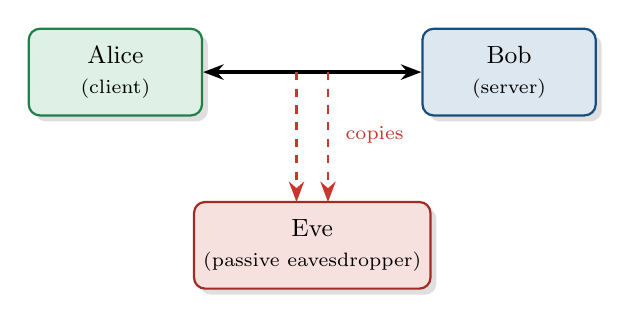
\begin{tikzpicture}
        \node[box=leaf,minimum width=22mm,minimum height=11mm] (al) at (0,0) {Alice\\\scriptsize(client)};
        \node[box=ocean,minimum width=22mm,minimum height=11mm] (bo) at (5,0) {Bob\\\scriptsize(server)};
        \draw[<->,very thick] (al) -- (bo);
        \node[box=brick,minimum width=26mm,minimum height=11mm] (ev) at (2.5,-2.2) {Eve\\\scriptsize(passive eavesdropper)};
        \draw[brick,dashed,thick,->] (2.3,0) -- (2.3,-1.65);
        \draw[brick,dashed,thick,->] (2.7,0) -- (2.7,-1.65);
        \node[font=\scriptsize,text=brick,anchor=west] at (2.8,-0.8) {copies};
      \end{tikzpicture}
    \end{column}
    \begin{column}{0.46\textwidth}
      \begin{itemize}\small\setlength{\itemsep}{4pt}
        \item An unauthorized attacker \textbf{monitors or listens} to the communication
        \item The goal is to \textbf{obtain information}
        \item Two kinds: \textbf{release of message contents} and \textbf{traffic analysis}
      \end{itemize}
      \vspace{2mm}
      \begin{block}{Hard to detect, easy to prevent}
        \small No data is altered, so passive attacks are very \textbf{difficult to detect}; but encryption makes them feasible to \textbf{prevent}.
      \end{block}
    \end{column}
  \end{columns}
\end{frame}

% ------------------------------------------------------------
\begin{frame}{Active Attacks: The Four Categories}
  \centering
  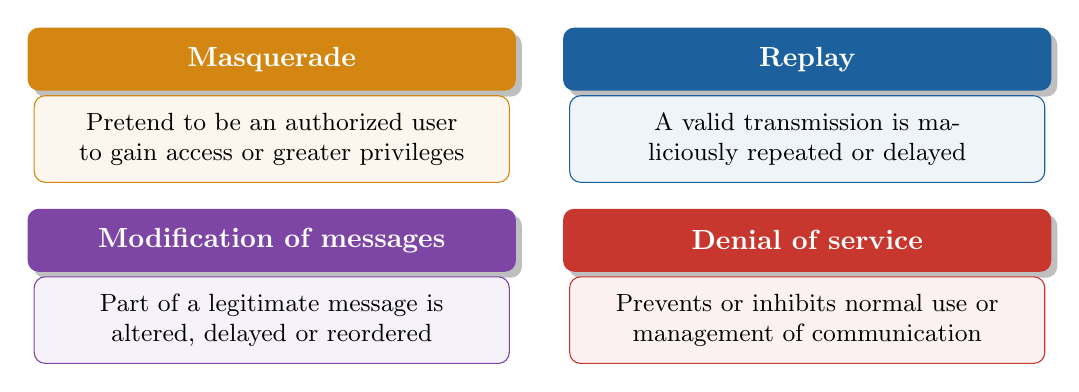
\begin{tikzpicture}
    \foreach \x/\y/\c/\t/\d in {
      0/0/amber!90!black/Masquerade/Pretend to be an authorized user to gain access or greater privileges,
      6.8/0/ocean/Replay/A valid transmission is maliciously repeated or delayed,
      0/-2.3/grape/Modification of messages/Part of a legitimate message is altered\comma{} delayed or reordered,
      6.8/-2.3/brick/Denial of service/Prevents or inhibits normal use or management of communication}
    {
      \node[fill=\c,text=white,rounded corners=4pt,font=\bfseries,minimum width=62mm,minimum height=8mm,drop shadow] (h) at (\x,\y) {\t};
      \node[draw=\c,fill=\c!7,rounded corners=4pt,text width=58mm,minimum height=11mm,align=center,font=\small,anchor=north] at ([yshift=-0.5mm]h.south) {\d};
    }
  \end{tikzpicture}
  \vspace{3mm}
  \begin{alertblock}{Common feature}
    \small Active attacks involve some \textbf{modification of the data stream} or the \textbf{creation of a false stream}.
  \end{alertblock}
\end{frame}

% ------------------------------------------------------------
\begin{frame}{Masquerade and Replay in Detail}
  \begin{columns}[T]
    \begin{column}{0.49\textwidth}
      \begin{block}{Masquerade}
        \small
        \begin{itemize}\setlength{\itemsep}{1pt}
          \item Uses \textbf{stolen logon IDs and passwords}, security gaps, or bypasses authentication
          \item May come from \textbf{inside} the organization or from outside
          \item \textbf{Weak authentication} is the easiest entry point
          \item Once in, the attacker may modify or delete data and change network configuration
        \end{itemize}
      \end{block}
    \end{column}
    \begin{column}{0.49\textwidth}
      \centering
      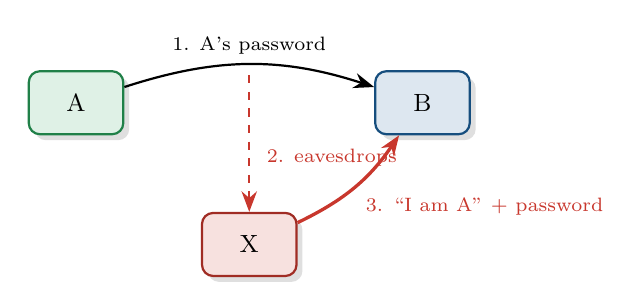
\begin{tikzpicture}
        \node[box=leaf,minimum width=12mm] (a) at (0,0) {A};
        \node[box=ocean,minimum width=12mm] (b) at (4.4,0) {B};
        \draw[->,thick] (a) to[bend left=18] node[above,font=\scriptsize]{1. A's password} (b);
        \node[box=brick,minimum width=12mm] (x) at (2.2,-1.8) {X};
        \draw[->,brick,dashed,thick] (2.2,0.35) -- (x);
        \node[font=\scriptsize,text=brick,anchor=west] at (2.3,-0.7) {2. eavesdrops};
        \draw[->,brick,very thick] (x) to[bend right=15] node[below right,font=\scriptsize]{3. ``I am A'' + password} (b);
      \end{tikzpicture}
      \begin{block}{Replay}
        \small X keeps A's password from the last session and sends it to B later. B \textbf{must accept} it.
      \end{block}
    \end{column}
  \end{columns}
\end{frame}

% ------------------------------------------------------------
\begin{frame}{Modification and Denial of Service in Detail}
  \begin{columns}[T]
    \begin{column}{0.49\textwidth}
      \begin{block}{Modification of messages}
        \small A message is altered, \textbf{delayed or reordered} to produce an unauthorized effect.
      \end{block}
      \centering
      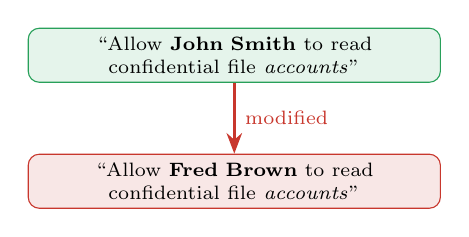
\begin{tikzpicture}
        \node[fill=leaf!12,draw=leaf,rounded corners,font=\scriptsize,text width=50mm,align=center] (o) at (0,0) {``Allow \textbf{John Smith} to read confidential file \textit{accounts}''};
        \node[fill=brick!12,draw=brick,rounded corners,font=\scriptsize,text width=50mm,align=center] (m) at (0,-1.6) {``Allow \textbf{Fred Brown} to read confidential file \textit{accounts}''};
        \draw[->,very thick,brick] (o) -- node[right,font=\scriptsize]{modified} (m);
      \end{tikzpicture}
    \end{column}
    \begin{column}{0.49\textwidth}
      \begin{alertblock}{Denial of service}
        \small Prevents or inhibits the normal use or management of communication facilities.
      \end{alertblock}
      \centering
      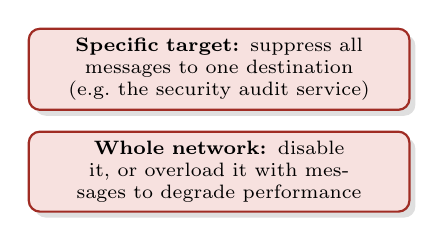
\begin{tikzpicture}
        \node[box=brick,minimum width=48mm,font=\scriptsize,text width=46mm,align=center] at (0,0) {\textbf{Specific target:} suppress all messages to one destination (e.g.\ the security audit service)};
        \node[box=brick,minimum width=48mm,font=\scriptsize,text width=46mm,align=center] at (0,-1.3) {\textbf{Whole network:} disable it, or overload it with messages to degrade performance};
      \end{tikzpicture}
    \end{column}
  \end{columns}
\end{frame}

% ------------------------------------------------------------
\begin{frame}{Passive vs. Active: What Should We Do?}
  \centering
  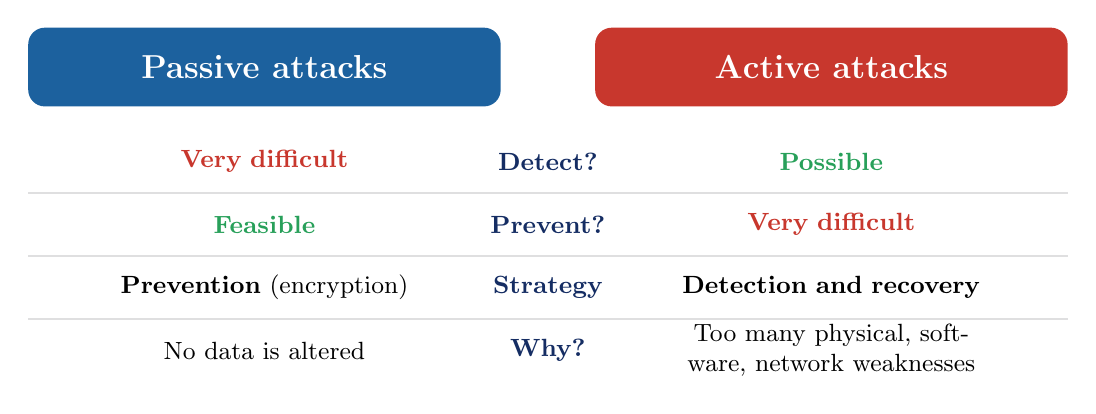
\begin{tikzpicture}
    \node[fill=ocean,text=white,rounded corners=6pt,minimum width=60mm,minimum height=10mm,font=\large\bfseries] (p) at (0,0) {Passive attacks};
    \node[fill=brick,text=white,rounded corners=6pt,minimum width=60mm,minimum height=10mm,font=\large\bfseries] (a) at (7.2,0) {Active attacks};
    \foreach \y/\l/\pv/\av in {-1.2/Detect?/\bad{Very difficult}/\good{Possible},
                              -2.0/Prevent?/\good{Feasible}/\bad{Very difficult},
                              -2.8/Strategy/\textbf{Prevention} (encryption)/\textbf{Detection and recovery},
                              -3.6/Why?/No data is altered/Too many physical\comma{} software\comma{} network weaknesses}{
      \node[font=\small\bfseries,text=navy] at (3.6,\y) {\l};
      \node[font=\small,text width=52mm,align=center] at (0,\y) {\pv};
      \node[font=\small,text width=52mm,align=center] at (7.2,\y) {\av};
    }
    \foreach \y in {-1.6,-2.4,-3.2} \draw[ink!15] (-3,\y) -- (10.2,\y);
  \end{tikzpicture}
  \vspace{3mm}
  \begin{exampleblock}{Bonus}
    \small If detection has a \textbf{deterrent effect}, it also contributes to preventing active attacks.
  \end{exampleblock}
\end{frame}

% ------------------------------------------------------------
\begin{frame}{The Six Security Services}
  \begin{columns}[c]
    \begin{column}{0.5\textwidth}
      \centering
      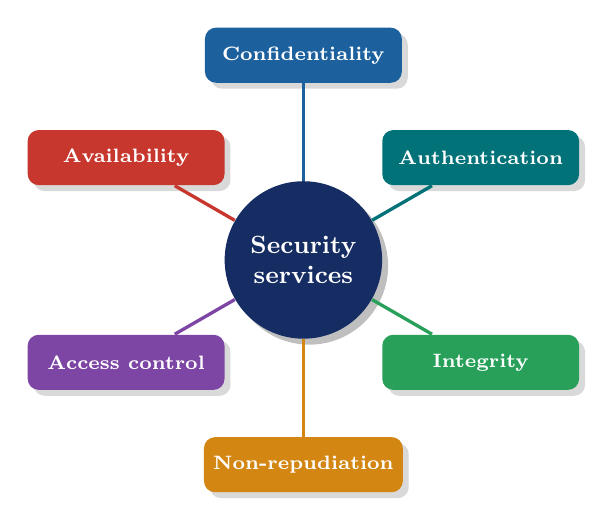
\begin{tikzpicture}
        \node[circle,fill=navy,text=white,font=\small\bfseries,minimum size=20mm,align=center,drop shadow] (c) at (0,0) {Security\\services};
        \foreach \a/\t/\c in {90/Confidentiality/ocean,30/Authentication/aqua!80!black,-30/Integrity/leaf,-90/Non-repudiation/amber!90!black,-150/Access control/grape,150/Availability/brick}{
          \node[solid box=\c,minimum width=25mm,minimum height=7mm,font=\scriptsize\bfseries] (s\a) at (\a:2.6) {\t};
          \draw[\c,very thick] (c) -- (s\a);
        }
      \end{tikzpicture}
    \end{column}
    \begin{column}{0.48\textwidth}
      \begin{block}{What is a security service?}
        \small A \textbf{base-level service} used to combat security attacks.
      \end{block}
      \vspace{2mm}
      \begin{alertblock}{Do not confuse}
        \small Services are \textbf{not} mechanisms. Mechanisms are the \textbf{actual implementations} of these services.
      \end{alertblock}
      \vspace{2mm}
      {\small The next slides take each service in turn.}
    \end{column}
  \end{columns}
\end{frame}

% ------------------------------------------------------------
\begin{frame}{Service 1: Confidentiality}
  \begin{columns}[c]
    \begin{column}{0.52\textwidth}
      \centering
      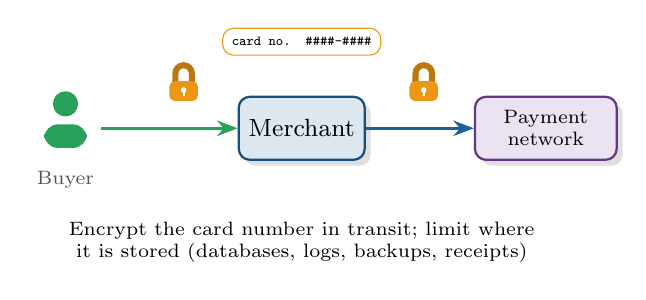
\begin{tikzpicture}
        \pic at (0,0) {person=leaf}; \node[tag] at (0,-0.5) {Buyer};
        \node[box=ocean,minimum width=16mm] (m) at (3,0.15) {Merchant};
        \node[box=grape,minimum width=18mm,font=\scriptsize] (p) at (6.1,0.15) {Payment\\network};
        \draw[flow=leaf] (0.45,0.15) -- (m); \draw[flow=ocean] (m) -- (p);
        \pic[scale=0.7] at (1.5,0.65) {lock=amber}; \pic[scale=0.7] at (4.55,0.65) {lock=amber};
        \node[fill=white,draw=amber,rounded corners,font=\tiny\ttfamily] at (3,1.25) {card no. \#\#\#\#-\#\#\#\#};
        \node[font=\scriptsize,text width=60mm,align=center] at (3,-1.3) {Encrypt the card number in transit; limit where it is stored (databases, logs, backups, receipts)};
      \end{tikzpicture}
    \end{column}
    \begin{column}{0.46\textwidth}
      \begin{itemize}\small\setlength{\itemsep}{3pt}
        \item Provides \textbf{secrecy}: only authorized users can access information
        \item Works with \textbf{accountability} to identify individuals
        \item Protects data in \textbf{paper files, electronic files, and in transit}
      \end{itemize}
      \vspace{1mm}
      \begin{alertblock}{Breaches of confidentiality}
        \scriptsize Someone reading your screen over your shoulder \,$\cdot$\, a stolen laptop with employee data \,$\cdot$\, giving information over the phone to an unauthorized caller
      \end{alertblock}
    \end{column}
  \end{columns}
\end{frame}

% ------------------------------------------------------------
\begin{frame}{Service 2: Authentication}
  \begin{columns}[c]
    \begin{column}{0.5\textwidth}
      \centering
      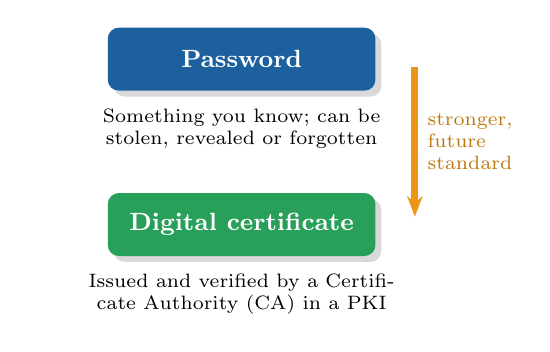
\begin{tikzpicture}
        \foreach \t/\c/\d [count=\i from 0] in {Password/ocean/Something you know; can be stolen\comma{} revealed or forgotten,
                                               Digital certificate/leaf/Issued and verified by a Certificate Authority (CA) in a PKI}{
          \node[solid box=\c,minimum width=34mm] (h\i) at (0,-\i*2.1) {\t};
          \node[font=\scriptsize,text width=52mm,align=center,below=1mm of h\i] {\d};
        }
        \draw[->,line width=2.5pt,amber] (2.2,-0.1) -- node[right,font=\scriptsize,text=amber!80!black,align=left]{stronger,\\future\\standard} (2.2,-2.0);
      \end{tikzpicture}
    \end{column}
    \begin{column}{0.48\textwidth}
      \begin{block}{Definition}
        \small Establishing or confirming that something (or someone) is \textbf{authentic}: claims made about it are true.
      \end{block}
      \begin{itemize}\small\setlength{\itemsep}{3pt}
        \item Confirms the identity of a \textbf{person}, the origin of an \textbf{artifact}, or that a \textbf{program} is trusted
        \item Commonly done with \textbf{logon passwords}
        \item Money transactions need a \textbf{more stringent} process
      \end{itemize}
    \end{column}
  \end{columns}
\end{frame}

% ------------------------------------------------------------
\begin{frame}{Service 3: Integrity}
  \begin{block}{Definition}
    \small The assurance that information can only be \textbf{accessed or modified by those authorized} to do so.
  \end{block}
  \vspace{2mm}
  \begin{columns}[T]
    \begin{column}{0.49\textwidth}
      \centering
      \textbf{\textcolor{leaf!70!black}{Connection-oriented integrity}}\\[2mm]
      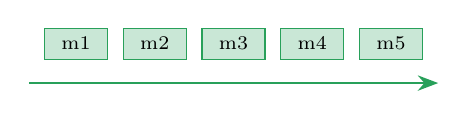
\begin{tikzpicture}
        \foreach \i in {1,...,5} \node[fill=leaf!25,draw=leaf,font=\scriptsize,minimum width=8mm] at (\i*1.0,0) {m\i};
        \draw[->,thick,leaf] (0.4,-0.5) -- (5.6,-0.5);
      \end{tikzpicture}\\[1mm]
      {\small A \textbf{stream} of messages is received as sent: no duplication, insertion, modification, reordering or replay. Also covers \textbf{destruction} of data.}
    \end{column}
    \begin{column}{0.49\textwidth}
      \centering
      \textbf{\textcolor{ocean}{Connectionless integrity}}\\[2mm]
      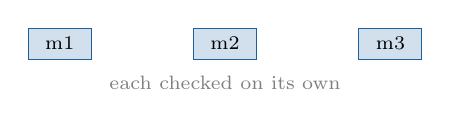
\begin{tikzpicture}
        \foreach \i/\x in {1/0,2/2.1,3/4.2} \node[fill=ocean!20,draw=ocean,font=\scriptsize,minimum width=8mm] at (\x,0) {m\i};
        \node[font=\scriptsize,text=ink!60] at (2.1,-0.5) {each checked on its own};
      \end{tikzpicture}\\[1mm]
      {\small Handles \textbf{individual messages} with no regard to larger context. Protects against \textbf{message modification only}.}
    \end{column}
  \end{columns}
\end{frame}

% ------------------------------------------------------------
\begin{frame}{Service 4: Non-Repudiation}
  \begin{columns}[c]
    \begin{column}{0.5\textwidth}
      \centering
      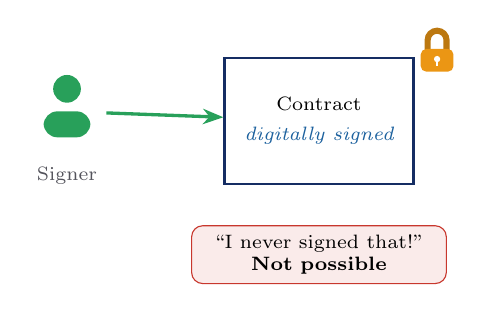
\begin{tikzpicture}
        \pic[scale=1.1] at (0,0) {person=leaf}; \node[tag] at (0,-0.6) {Signer};
        \node[draw=navy,fill=white,thick,minimum width=24mm,minimum height=16mm,font=\scriptsize,align=center] (d) at (3.2,0.1) {Contract\\[3pt]\textit{\textcolor{ocean}{digitally signed}}};
        \draw[flow=leaf] (0.5,0.2) -- (d);
        \node[fill=brick!10,draw=brick,rounded corners,font=\scriptsize,text width=30mm,align=center] at (3.2,-1.6) {``I never signed that!''\\\textbf{Not possible}};
        \pic[scale=0.8] at (4.7,0.9) {lock=amber};
      \end{tikzpicture}
    \end{column}
    \begin{column}{0.48\textwidth}
      \begin{block}{Definition}
        \small A party to a contract or communication \textbf{cannot deny} the authenticity of its signature or of sending a message it originated.
      \end{block}
      \begin{itemize}\small\setlength{\itemsep}{3pt}
        \item A \textbf{digital signature} proves who signed, and can be created by \textbf{only one person}
        \item No technology is fool-proof, so add \textbf{biometrics}, time stamps, printed receipts
      \end{itemize}
    \end{column}
  \end{columns}
\end{frame}

% ------------------------------------------------------------
\begin{frame}{Services 5 \& 6: Access Control and Availability}
  \begin{columns}[T]
    \begin{column}{0.49\textwidth}
      \begin{block}{Access control}
        \small The ability to \textbf{permit or deny} the use of a resource by a particular entity.
      \end{block}
      \centering
      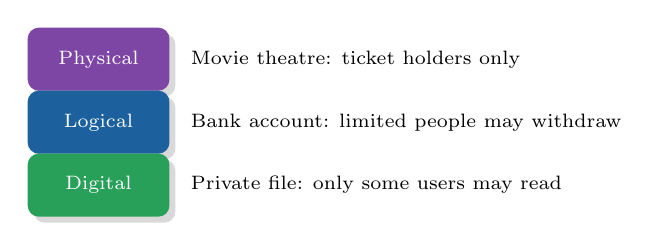
\begin{tikzpicture}
        \foreach \t/\e/\c [count=\i from 0] in {Physical/Movie theatre: ticket holders only/grape,Logical/Bank account: limited people may withdraw/ocean,Digital/Private file: only some users may read/leaf}{
          \node[solid box=\c,minimum width=18mm,font=\scriptsize] at (0,-\i*0.8) {\t};
          \node[anchor=west,font=\scriptsize] at (1.05,-\i*0.8) {\e};
        }
      \end{tikzpicture}
    \end{column}
    \begin{column}{0.49\textwidth}
      \begin{alertblock}{Availability}
        \small A system or resource is \textbf{accessible and usable on demand} by an authorized entity, per its specifications.
      \end{alertblock}
      \begin{itemize}\small\setlength{\itemsep}{3pt}
        \item Network, hardware and software are \textbf{reliable}
        \item They \textbf{recover quickly} after an interruption
        \item They should resist \textbf{denial-of-service} attacks
      \end{itemize}
    \end{column}
  \end{columns}
\end{frame}

% ------------------------------------------------------------
\begin{frame}{Which Service Fights Which Attack?}
  \centering
  \renewcommand{\arraystretch}{1.35}
  \small
  \begin{tabular}{l c c c c c c}
    \toprule
    \rowcolor{navy} & \textcolor{white}{\textbf{Confid.}} & \textcolor{white}{\textbf{Auth.}} & \textcolor{white}{\textbf{Integrity}} & \textcolor{white}{\textbf{Non-rep.}} & \textcolor{white}{\textbf{Access}} & \textcolor{white}{\textbf{Avail.}}\\
    \midrule
    \textbf{Release of contents} & \good{\checkmark} & & & & \good{\checkmark} & \\
    \textbf{Traffic analysis}    & \good{\checkmark} & & & & & \\
    \textbf{Masquerade}          & & \good{\checkmark} & & & \good{\checkmark} & \\
    \textbf{Replay}              & & \good{\checkmark} & \good{\checkmark} & & & \\
    \textbf{Modification}        & & & \good{\checkmark} & \good{\checkmark} & & \\
    \textbf{Denial of service}   & & & & & & \good{\checkmark}\\
    \bottomrule
  \end{tabular}
  \vspace{4mm}

  
\begin{tikzpicture}
    \node[fill=sky,rounded corners,text width=12cm,align=center,font=\small,inner sep=6pt]
      {Every attack is answered by at least one service, and each service is built from mechanisms (Modules 6--12).};
  \end{tikzpicture}
\end{frame}

% ------------------------------------------------------------
\begin{frame}{A Model for Network Security}
  \centering
  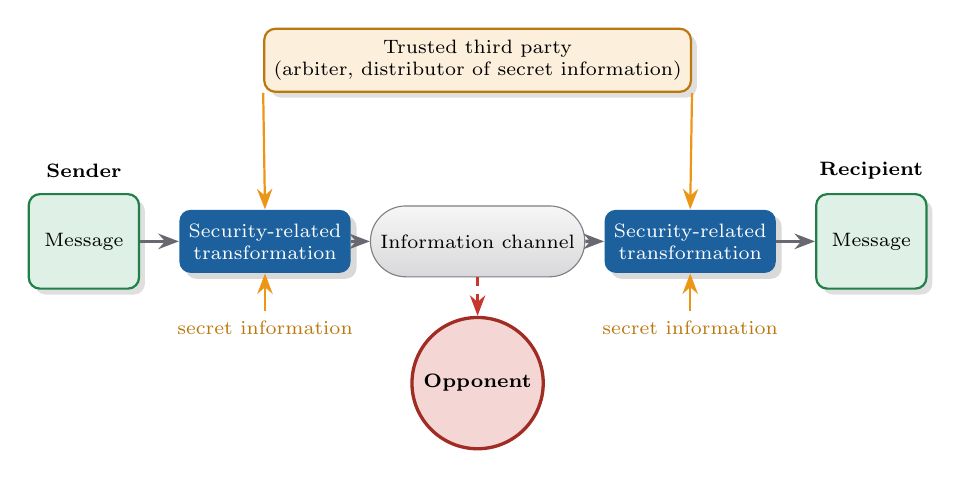
\begin{tikzpicture}
    \node[box=amber,minimum width=44mm,font=\scriptsize] (ttp) at (5,2.3) {Trusted third party\\(arbiter, distributor of secret information)};
    \node[box=leaf,minimum width=14mm,minimum height=12mm,font=\scriptsize] (msg) at (0,0) {Message};
    \node[solid box=ocean,minimum width=20mm,font=\scriptsize] (t1) at (2.3,0) {Security-related\\transformation};
    \node[draw=ink!60,top color=ink!4,bottom color=ink!18,rounded rectangle,minimum width=26mm,minimum height=9mm,font=\scriptsize] (ch) at (5,0) {Information channel};
    \node[solid box=ocean,minimum width=20mm,font=\scriptsize] (t2) at (7.7,0) {Security-related\\transformation};
    \node[box=leaf,minimum width=14mm,minimum height=12mm,font=\scriptsize] (msg2) at (10,0) {Message};
    \draw[flow] (msg) -- (t1); \draw[flow] (t1) -- (ch); \draw[flow] (ch) -- (t2); \draw[flow] (t2) -- (msg2);
    \node[font=\scriptsize,text=amber!80!black] (s1) at (2.3,-1.1) {secret information};
    \node[font=\scriptsize,text=amber!80!black] (s2) at (7.7,-1.1) {secret information};
    \draw[->,amber,thick] (s1) -- (t1); \draw[->,amber,thick] (s2) -- (t2);
    \draw[->,amber,thick] (ttp.south west) -- (t1.north); \draw[->,amber,thick] (ttp.south east) -- (t2.north);
    \node[font=\scriptsize\bfseries] at (0,0.9) {Sender}; \node[font=\scriptsize\bfseries] at (10,0.9) {Recipient};
    \node[station=brick,minimum size=11mm,font=\scriptsize\bfseries] (op) at (5,-1.8) {Opponent};
    \draw[brick,dashed,thick,->] (ch.south) -- (op);
  \end{tikzpicture}
  \vspace{1mm}
  \begin{itemize}\footnotesize
    \item Two \textbf{principals} cooperate over a logical channel (a route through the Internet using protocols such as TCP/IP)
    \item Security = a \textbf{transformation} of the message (e.g. encryption) + \textbf{secret information} shared by the two (e.g. a key)
  \end{itemize}
\end{frame}

% ------------------------------------------------------------
\begin{frame}{Four Basic Tasks in Designing a Security Service}
  \centering
  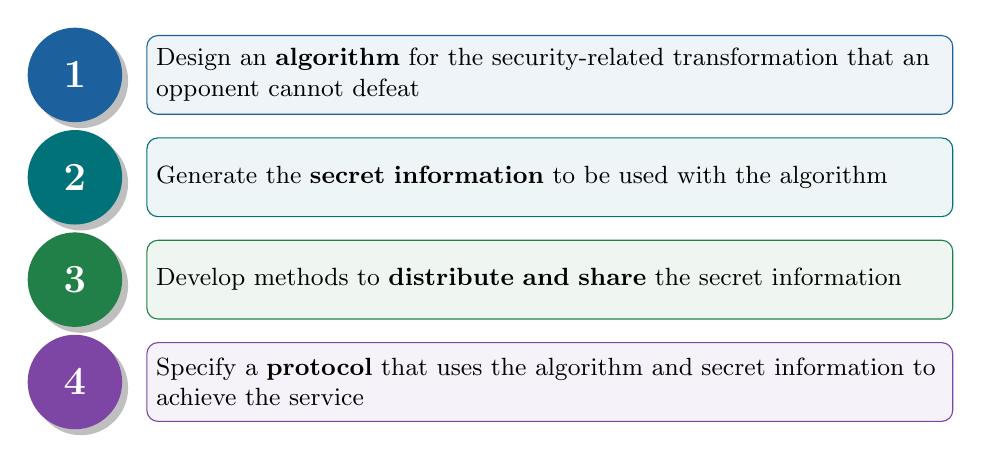
\begin{tikzpicture}
    \foreach \t/\c [count=\i] in {
      {Design an \textbf{algorithm} for the security-related transformation that an opponent cannot defeat}/ocean,
      {Generate the \textbf{secret information} to be used with the algorithm}/aqua!80!black,
      {Develop methods to \textbf{distribute and share} the secret information}/leaf!80!black,
      {Specify a \textbf{protocol} that uses the algorithm and secret information to achieve the service}/grape}
    {
      \node[circle,fill=\c,text=white,font=\Large\bfseries,minimum size=12mm,drop shadow] (c\i) at (0,-\i*1.3) {\i};
      \node[draw=\c,fill=\c!7,rounded corners=4pt,anchor=west,text width=100mm,minimum height=10mm,font=\small] at ([xshift=3mm]c\i.east) {\t};
    }
  \end{tikzpicture}
  \vspace{2mm}

  {\small A \textbf{trusted third party} may distribute the secret information or settle disputes between the principals.}
\end{frame}

% ------------------------------------------------------------
\begin{frame}{The Network Access Security Model}
  \centering
  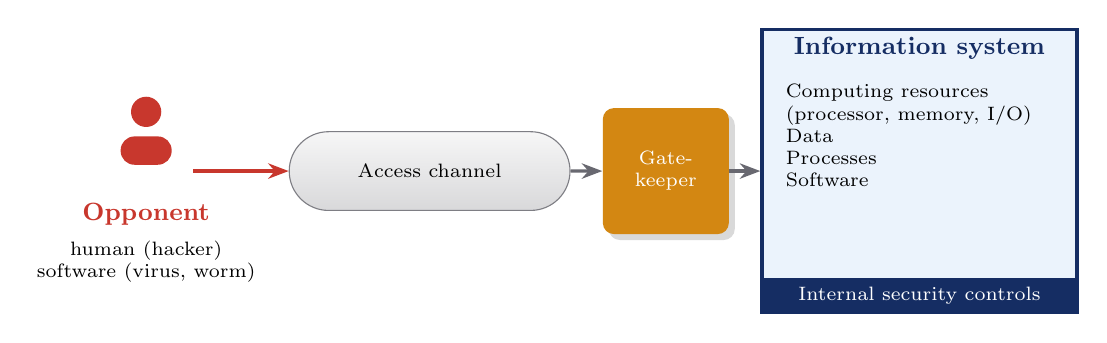
\begin{tikzpicture}
    \pic[scale=1.2] at (0,0.4) {person=brick};
    \node[font=\small\bfseries,text=brick] at (0,-0.35) {Opponent};
    \node[font=\scriptsize,align=center] at (0,-0.95) {human (hacker)\\software (virus, worm)};
    \node[draw=ink!60,top color=ink!4,bottom color=ink!18,rounded rectangle,minimum width=38mm,minimum height=10mm,font=\scriptsize] (ch) at (3.6,0.2) {Access channel};
    \node[solid box=amber!90!black,minimum width=16mm,minimum height=16mm,font=\scriptsize,align=center] (gk) at (6.6,0.2) {Gate-\\keeper};
    \draw[flow=brick] (0.6,0.2) -- (ch);
    \draw[flow] (ch) -- (gk);
    \node[draw=navy,very thick,fill=sky,minimum width=40mm,minimum height=36mm,anchor=west] (is) at (7.8,0.2) {};
    \node[font=\small\bfseries,text=navy,anchor=north] at (is.north) {Information system};
    \node[font=\scriptsize,align=left,anchor=north west] at ([xshift=2mm,yshift=-6mm]is.north west) {Computing resources\\(processor, memory, I/O)\\Data\\Processes\\Software};
    \node[fill=navy,text=white,font=\scriptsize,minimum width=40mm,anchor=south] at (is.south) {Internal security controls};
    \draw[flow] (gk) -- (is.west);
  \end{tikzpicture}
  \vspace{2mm}
  \begin{itemize}\small
    \item Protects an information system from \textbf{unwanted access}
    \item \textbf{Gatekeeper function}: password logins, screening programs; then \textbf{internal controls} watch activity inside
  \end{itemize}
\end{frame}

% ------------------------------------------------------------
\begin{frame}{Who Are the Intruders? What Do They Threaten?}
  \begin{columns}[T]
    \begin{column}{0.49\textwidth}
      \centering\textbf{\textcolor{brick}{Intruders}}\\[2mm]
      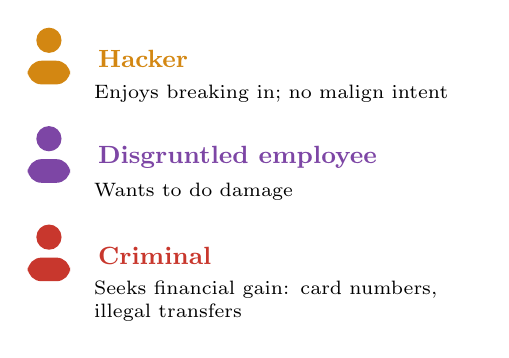
\begin{tikzpicture}
        \foreach \t/\d/\c [count=\i from 0] in {Hacker/Enjoys breaking in; no malign intent/amber!90!black,Disgruntled employee/Wants to do damage/grape,Criminal/Seeks financial gain: card numbers\comma{} illegal transfers/brick}{
          \pic at (0,-\i*1.25) {person=\c};
          \node[anchor=west,font=\small\bfseries,text=\c] at (0.5,-\i*1.25+0.22) {\t};
          \node[anchor=north west,font=\scriptsize,text width=48mm] at (0.45,-\i*1.25+0.02) {\d};
        }
      \end{tikzpicture}
    \end{column}
    \begin{column}{0.49\textwidth}
      \centering\textbf{\textcolor{navy}{Malicious logic}}\\[2mm]
      {\small Logic placed in a system to exploit vulnerabilities; it can affect applications and utility programs (editors, compilers).}\\[3mm]
      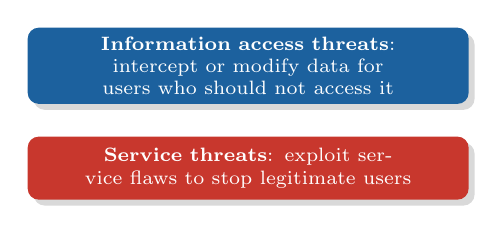
\begin{tikzpicture}
        \node[solid box=ocean,minimum width=56mm,font=\scriptsize,text width=52mm,align=center] at (0,0) {\textbf{Information access threats}: intercept or modify data for users who should not access it};
        \node[solid box=brick,minimum width=56mm,font=\scriptsize,text width=52mm,align=center] at (0,-1.3) {\textbf{Service threats}: exploit service flaws to stop legitimate users};
      \end{tikzpicture}
    \end{column}
  \end{columns}
\end{frame}

% ------------------------------------------------------------
\begin{frame}{Module 2 Summary}
  \begin{columns}[T]
    \begin{column}{0.49\textwidth}
      \begin{block}{Lesson 3: Types of Attacks}
        \small
        \begin{itemize}\setlength{\itemsep}{0pt}
          \item General view: criminal, publicity, legal
          \item Technical view: passive vs.\ active
          \item Masquerade, replay, alteration, DoS
          \item Application- vs.\ network-level attacks
          \item Viruses: 4 phases, 6 types
          \item 5 attacks on ciphers
        \end{itemize}
      \end{block}
    \end{column}
    \begin{column}{0.49\textwidth}
      \begin{exampleblock}{Lesson 9: Attacks, Services, Model}
        \small
        \begin{itemize}\setlength{\itemsep}{0pt}
          \item Passive: release of contents, traffic analysis
          \item Active: masquerade, replay, modification, DoS
          \item Six security services
          \item Model for network security; 4 tasks
          \item Network access security model
        \end{itemize}
      \end{exampleblock}
    \end{column}
  \end{columns}
  \vspace{1mm}
  \begin{alertblock}{Review questions}
    \scriptsize
    1.~Explain different types of attacks. \quad 2.~What are the possible types of attacks (on a cipher)? \quad
    3.~Write short notes on different types of security attacks. \quad 4.~Explain the model for network security. \quad
    5.~What are the different types of security services?
  \end{alertblock}
\end{frame}

% ------------------------------------------------------------
\begin{frame}{References}
  \begin{enumerate}\setlength{\itemsep}{8pt}
    \item William Stallings, \emph{Cryptography and Network Security}, PHI Publishers.
    \item Charlie Kaufman, Radia Perlman, \emph{Network Security}, Pearson Education.
    \item Bruce Schneier, \emph{Applied Cryptography}, John Wiley \& Sons.
    \item Roberta Bragg, \emph{Network Security: The Complete Reference}, TMH.
  \end{enumerate}
  \vspace{6mm}
  \centering
  
\begin{tikzpicture}
    \node[fill=navy,text=white,rounded corners=8pt,inner sep=10pt,font=\Large\bfseries,drop shadow] {Thank You! \; Questions?};
  \end{tikzpicture}
\end{frame}

\end{document}
